\chapter{Experiment}
This chapter describes the experimental setup in this study. The experiment is performed at Rare Isotope Beam Factory (RIBF) at RIKEN Nishina Center \cite{RIKEN}. A primary ${}^{48}$Ca beam is produced by the RIKEN accelerator complex and delivered to the BigRIPS separator \cite{Kubo03}\cite{Kubo07}\cite{Kubo12}. The BigRIPS separator produced the ${}^{17}$B secondary beam which bombarded on the lead and carbon targets in front of the SAMURAI (Superconducting Analyzer for MUlti-particles from Radioisotope beams) spectrometer\cite{SAMURAI}. After the reaction at the target, the fragments ${}^{15}$B and two neutrons are detected by detectors at SAMURAI system. 


\section{Beam Information}
The primary beam was accelerated by the SRC, RIBF. By accelerating ${}^{48}$Ca to 345 MeV/u and bombarding it on a thick Be target (30mm), a secondary beam was produced. The characteristics of the primary beam is in Table \ref{tab:Primary_Beam}.

    \begin{table}[h]
        \centering 
            \begin{tabular}[]{c|c|c|c}
                \hline
                Primary beam & Beam energy & Beam intensity & primary Target  \\
                \hline 
                ${}^{48}$Ca & 345 MeV/u & 210 pnA & Be (30mm)\\
                \hline    
            \end{tabular}
        \caption{Information of primary beam}
        \label{tab:Primary_Beam}
    \end{table}

The collision of the primary beam and the target created the secondary beam, including not only the purpose isotope of this experiment, ${}^{19}$B, but also other neighboring isotopes. The main isotope used in this research is ${}^{17}$B, which needed to be separated and identified through the BigRIPS separator. The identified ${}^{17}$B was then transferred to SAMURAI, where it underwent Coulomb dissociation, the main objective of this research. Three different targets were used: C, Pb, and Empty. The details for the secondary beam $^{17}$B is in Table \ref{tab:Secondary_Beam}.
\begin{table}[ht]
    \centering
    \begin{tabular}[ht]{c|c|c}
        \hline
        Isotope & Target & Average energy at the middle of target \\
        \hline
        & C (1.789 g/cm$^2$)  & 270 MeV/u\\
        ${}^{17}$B & Empty  & 275 MeV/u\\
        & Pb (3.255 g/cm$^2$) & 270 MeV/u\\
        \hline    
    \end{tabular}
    \caption{Information of secondary beam}
    \label{tab:Secondary_Beam}
\end{table}

\section{BigRIPS separator}

\begin{figure}[]
    \centering
    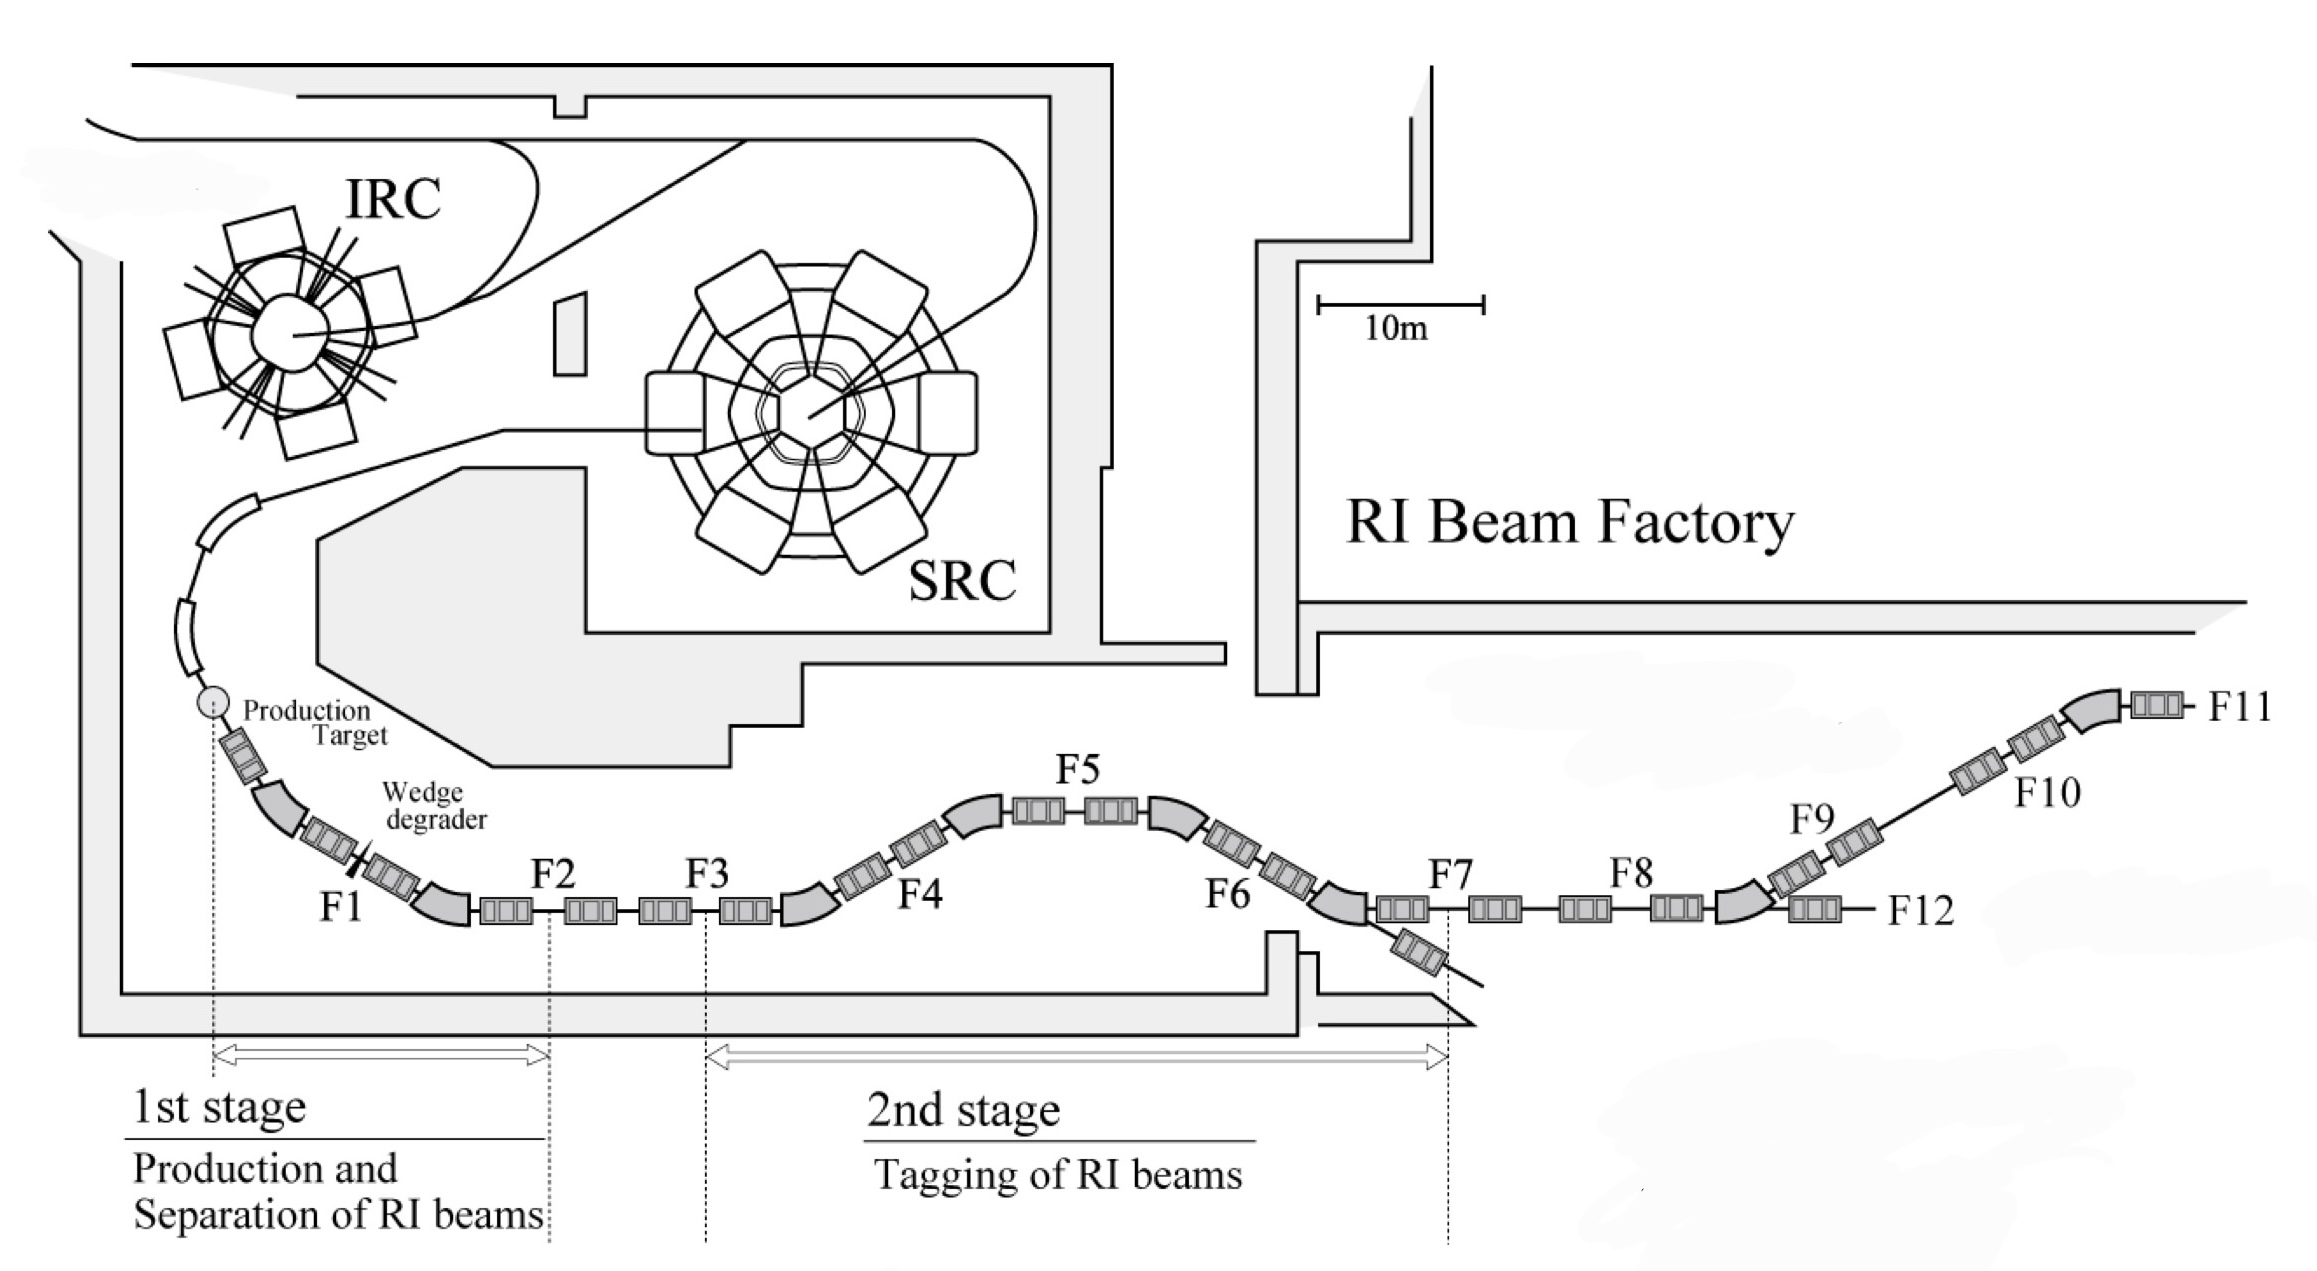
\includegraphics[width=12cm]{chapter3/BigRIPS_roof.jpg}
    \caption{A top view of the BigRIPS separator \cite{Dayonewiki}}
    \label{fig:BigRIPS}
\end{figure} 

The generated RI beams from SRC are separated by the BigRIPS separator. Figure \ref{fig:BigRIPS} shows a top view of the BigRIPS separator. In the first stage of BigRIPS separator, the RI beam separated by dipole magnet with slit and wedge-shaped degrader located at F1 focal plane. In the dipole magnet, the rigidity of a particle can be written as following eq (\ref{eq:rigidity}).
    \begin{align}
        B\rho = v \cdot \frac{A}{Z}  \label{eq:rigidity}
    \end{align}
The velocity of the secondary beam is almost same regardless of the nuclei so that it can be possible to choose specific $A/Z$ by adjusting the slit to filter only some $B\rho$ value. After that, the wedge-shaped degrader makes the beam energy depends on the $Z$ so that even same $A/Z$ nuclei can be separated. Table \ref{tab:BigRIPS} shows the BigRIPS separator setup for this experiment.

    \begin{table}[h]
        \centering
        \begin{tabular}{c c c c}
            \hline
            Location  & Slit[mm] & Degrader / Detector \\
            \hline
            F0  &  & Be target (30mm) \\
            F1  & $\pm$120 & Al wedge degrader (15mm)\\
            F2  & L: 10 R: 7 & \\
            F3   & & Plastic Scintillator (3mm)\\
            F5 & $\pm$120 & Beam Proportional Chamber \\
            F7  & $\pm$120 & Plastic Scintillator (3mm)\\
            F8  &$\pm$170 & \\
            F12 & $\pm$170 & \\
            %F13 &  & & Plastic Scintillator (0.5mm$\times$2)\\
            \hline
        \end{tabular}
        \caption{BigRIPS separator setup for Dayone experiment \cite{Dayonewiki}}
        \label{tab:BigRIPS}
    \end{table}
In the second stage, the RI beam is identified using TOF-B$\rho$-$\Delta E$ method. Detector information at BigRIPS will be described as following.

\subsection{Plastic Scintillator}
At focal plane F3, F7 and F13 in BigRIPS beam line, plastic scintillators are located for measuring the time of flight (TOF) of secondary beam. In F3 and F7, plastic scintillator with 3mm thickness is located and at F13 there are two scintillators, SBT1 and SBT2, with 0.5mm thickness. The flight length between F7 and F13 (Average point of SBTs) is 36.62 m. Table \ref{tab:Plastic_Scintillator} shows the information of plastic scintillators at F3, F7, and F13.

\begin{table}[h]
    \centering
    \begin{tabular}{c|cc}
        \hline
        Location & Thickness & Distance from target upstream \\
        \hline
        F3 & 3mm & 86.05 m\\
        F7 & 3mm & 39.48 m\\
        F13-1 &0.5mm & 2.90 m\\
        F13-2 &0.5mm & 2.82 m\\
        \hline
    \end{tabular}
    \caption{Information of plastic scintillators at F3, F7, F13}
    \label{tab:Plastic_Scintillator}
\end{table}

\section{SAMURAI}

\begin{figure}[hbt!]
    \centering
    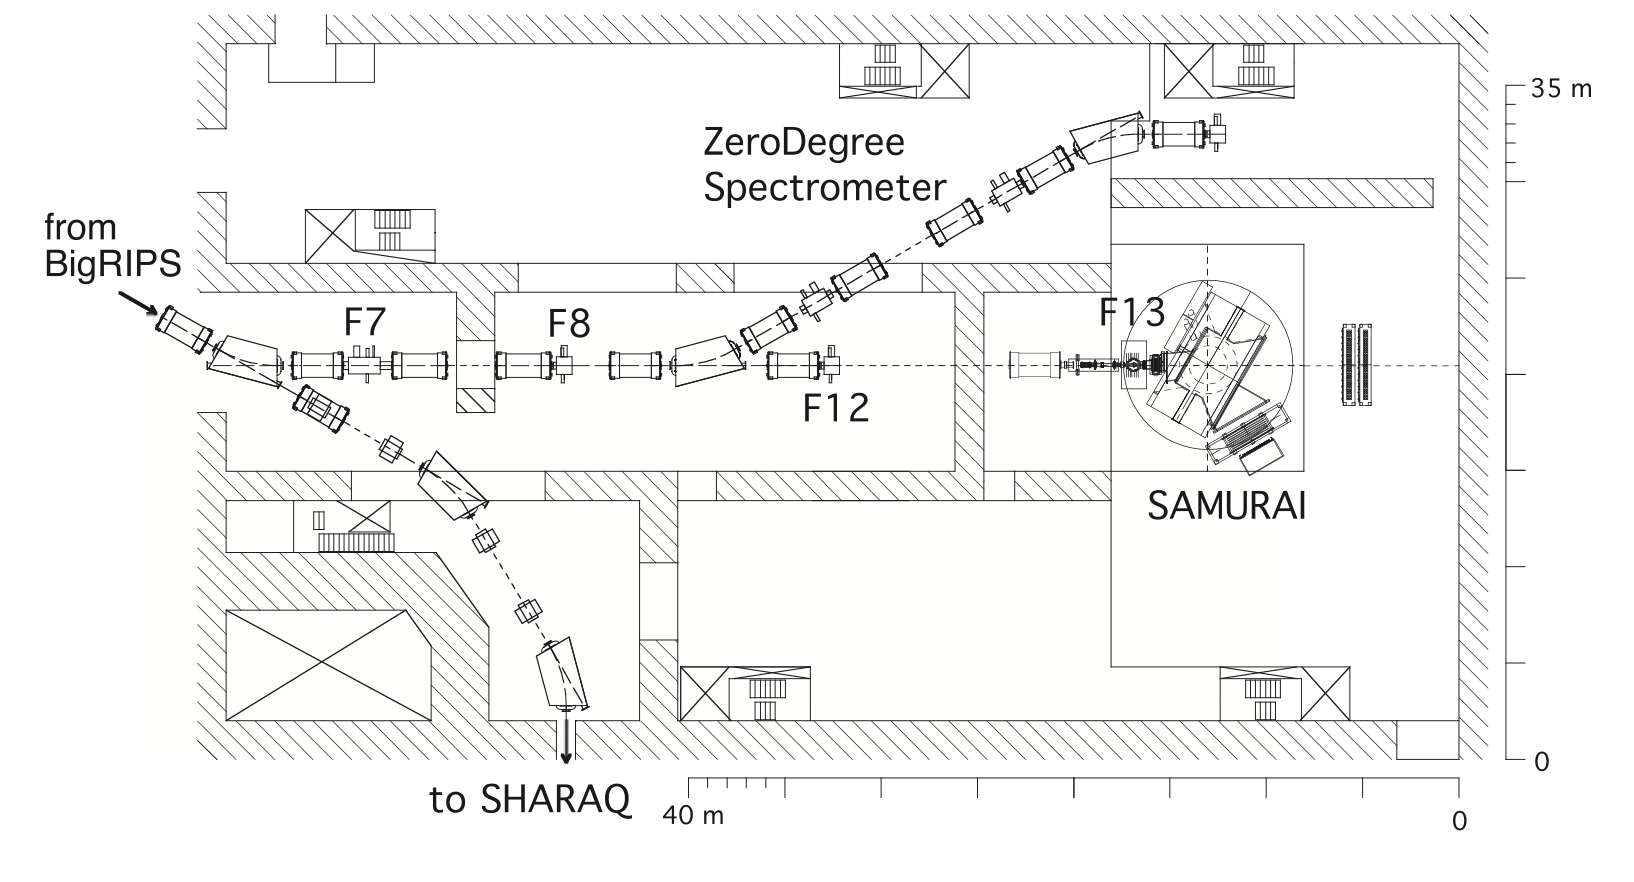
\includegraphics[width=8cm]{chapter3/SAMURAI1.png}
    \caption{A top view of the beam line from BigRIPS to SAMURAI spectrometer\cite{BigRIPSInfo}}
    \label{fig:BigRIPStoSAMURAI}
\end{figure}

The SAMURAI spectrometer is designed for kinematically complete experiment such as invariant mass spectroscopy\cite{SAMURAIConcept}. Figure \ref{fig:BigRIPStoSAMURAI} and \ref{fig:SAMURAI} shows a top view of the SAMURAI spectrometer. SAMURAI system includes Beam proportional chamber (BPC) for $B\rho$ measurement at F5, and two drift chambers (BDC1, BDC2) for tracking the secondary beam particle. After the reaction at secondary target, charged fragment bent by SAMURAI superconducting magnet and detected by two drift chambers (FDC1, FDC2) and one plastic scintillator (HODF). Finally the neutron detector array NEBULA is located at the end of extended beam line for neutron detection. The detailed information of each detector is described as following.

\begin{figure}[t]
    \centering
    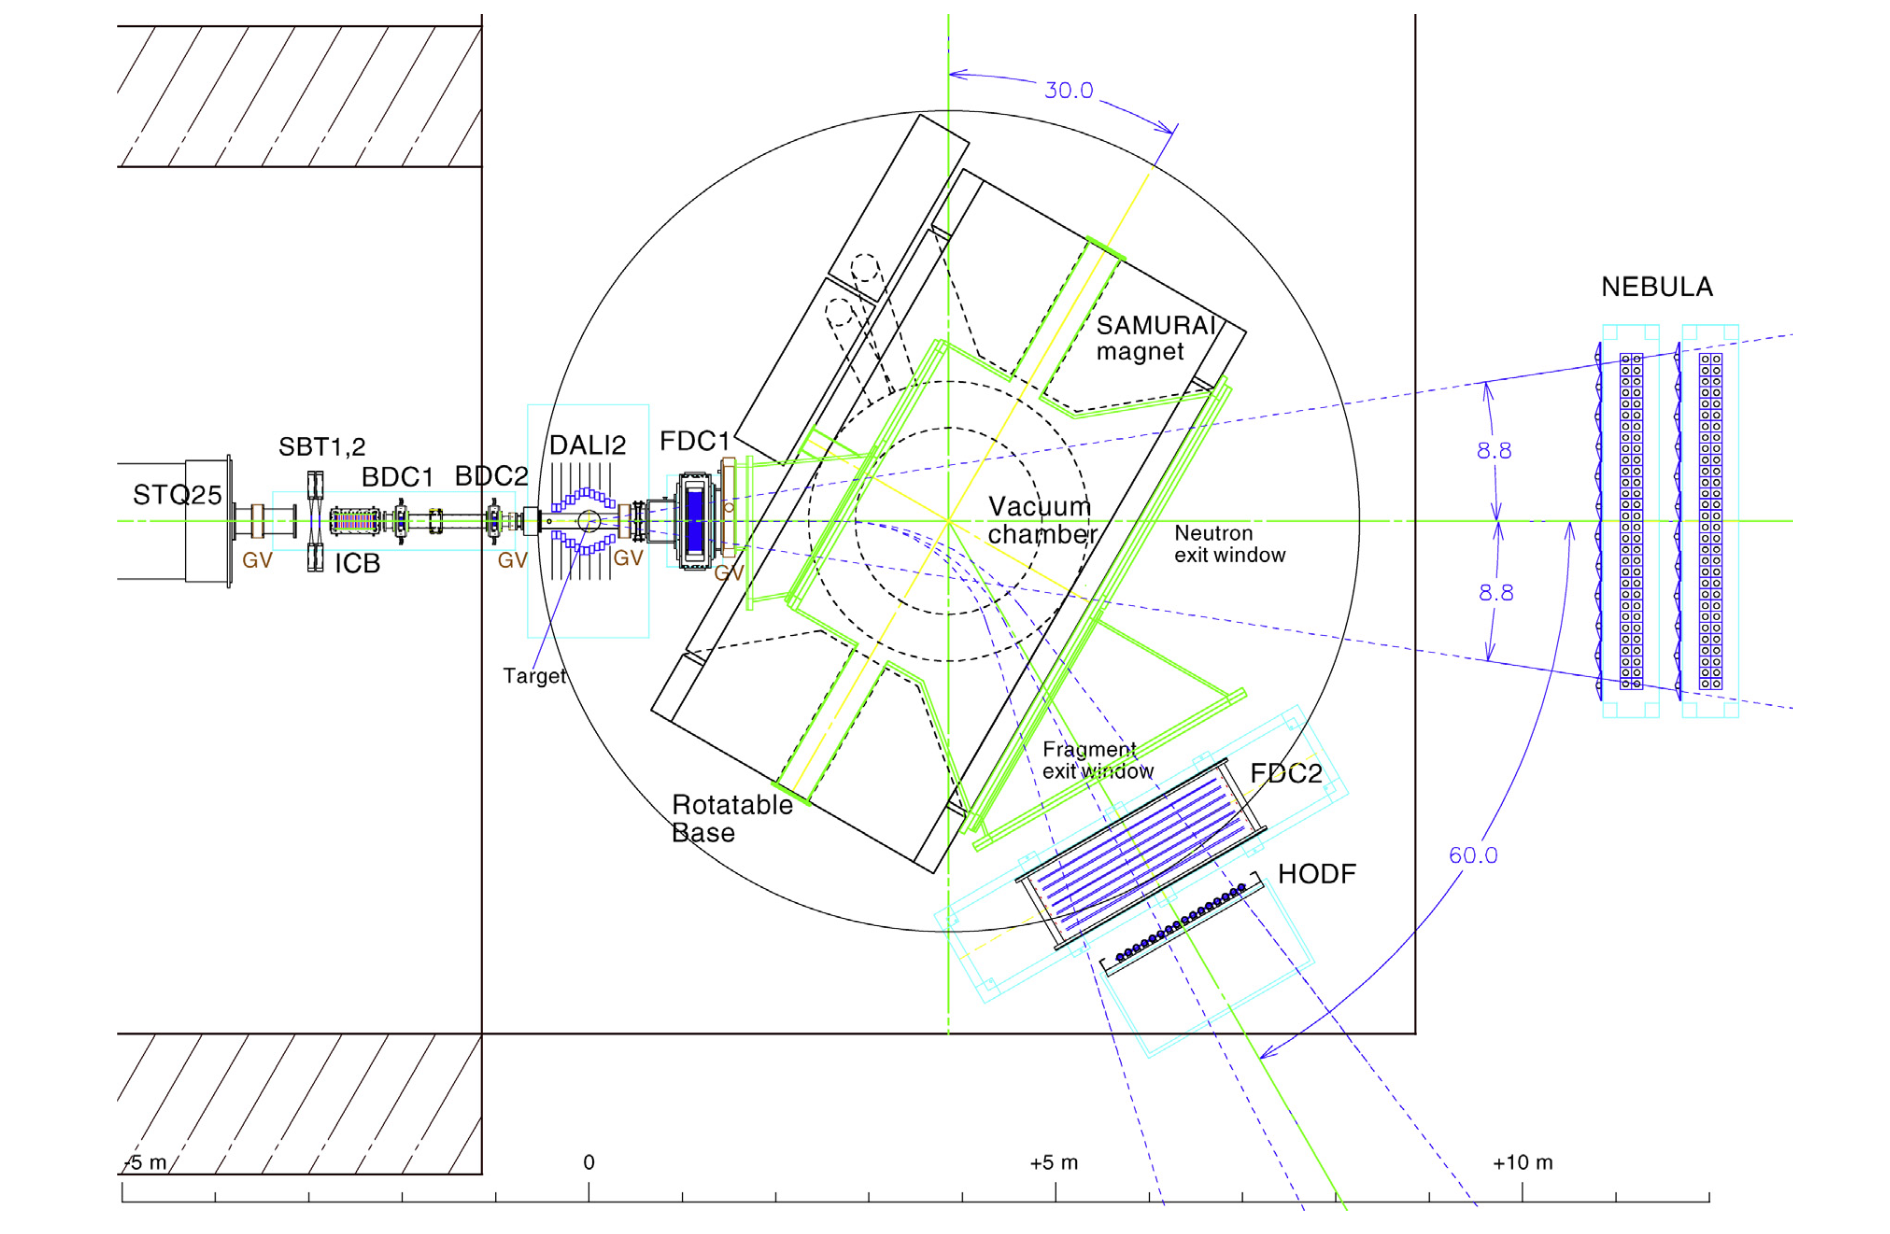
\includegraphics[width=\textwidth]{chapter3/SAMURAI.png}
    \caption{A top view of the SAMURAI spectrometer\cite{SAMURAI}}
    \label{fig:SAMURAI}
\end{figure}

\subsection{BPC (Beam Proportional Chamber)}
BPC is Multi Wire Proportional Chamber (MWPC) located at F5 focal plane which is used for measuring the position of beam. The purpose of BPC is tagging magnetic rigidity and momentum of secondary beam. Figure \ref{fig:BPC} shows the schematic view of BPC and Table \ref{tab:BPC} shows the parameter of BPC.
\begin{table}[h]
    \centering
    \begin{tabular}{l|c}
        \hline
        Effective Area & (H)240mm $\times$ (V)150mm \\
        Configuration & $XX$ (2 Planes) \\
        number of wire & 64 $\times$ 2 = 128 \\
        Wire Pitch & 4mm \\
        Gas & $i$--${\text{C}}_{4} {\text{H}}_{10}$ at 50 torr\\
        \hline
    \end{tabular}
    \caption{Parameter of BPC (Beam Proportional Chamber) \cite{SAMURAI}}
    \label{tab:BPC}
\end{table}

\begin{figure}[h]
    \centering
    \begin{subfigure}[h]{\textwidth}
        \centering
        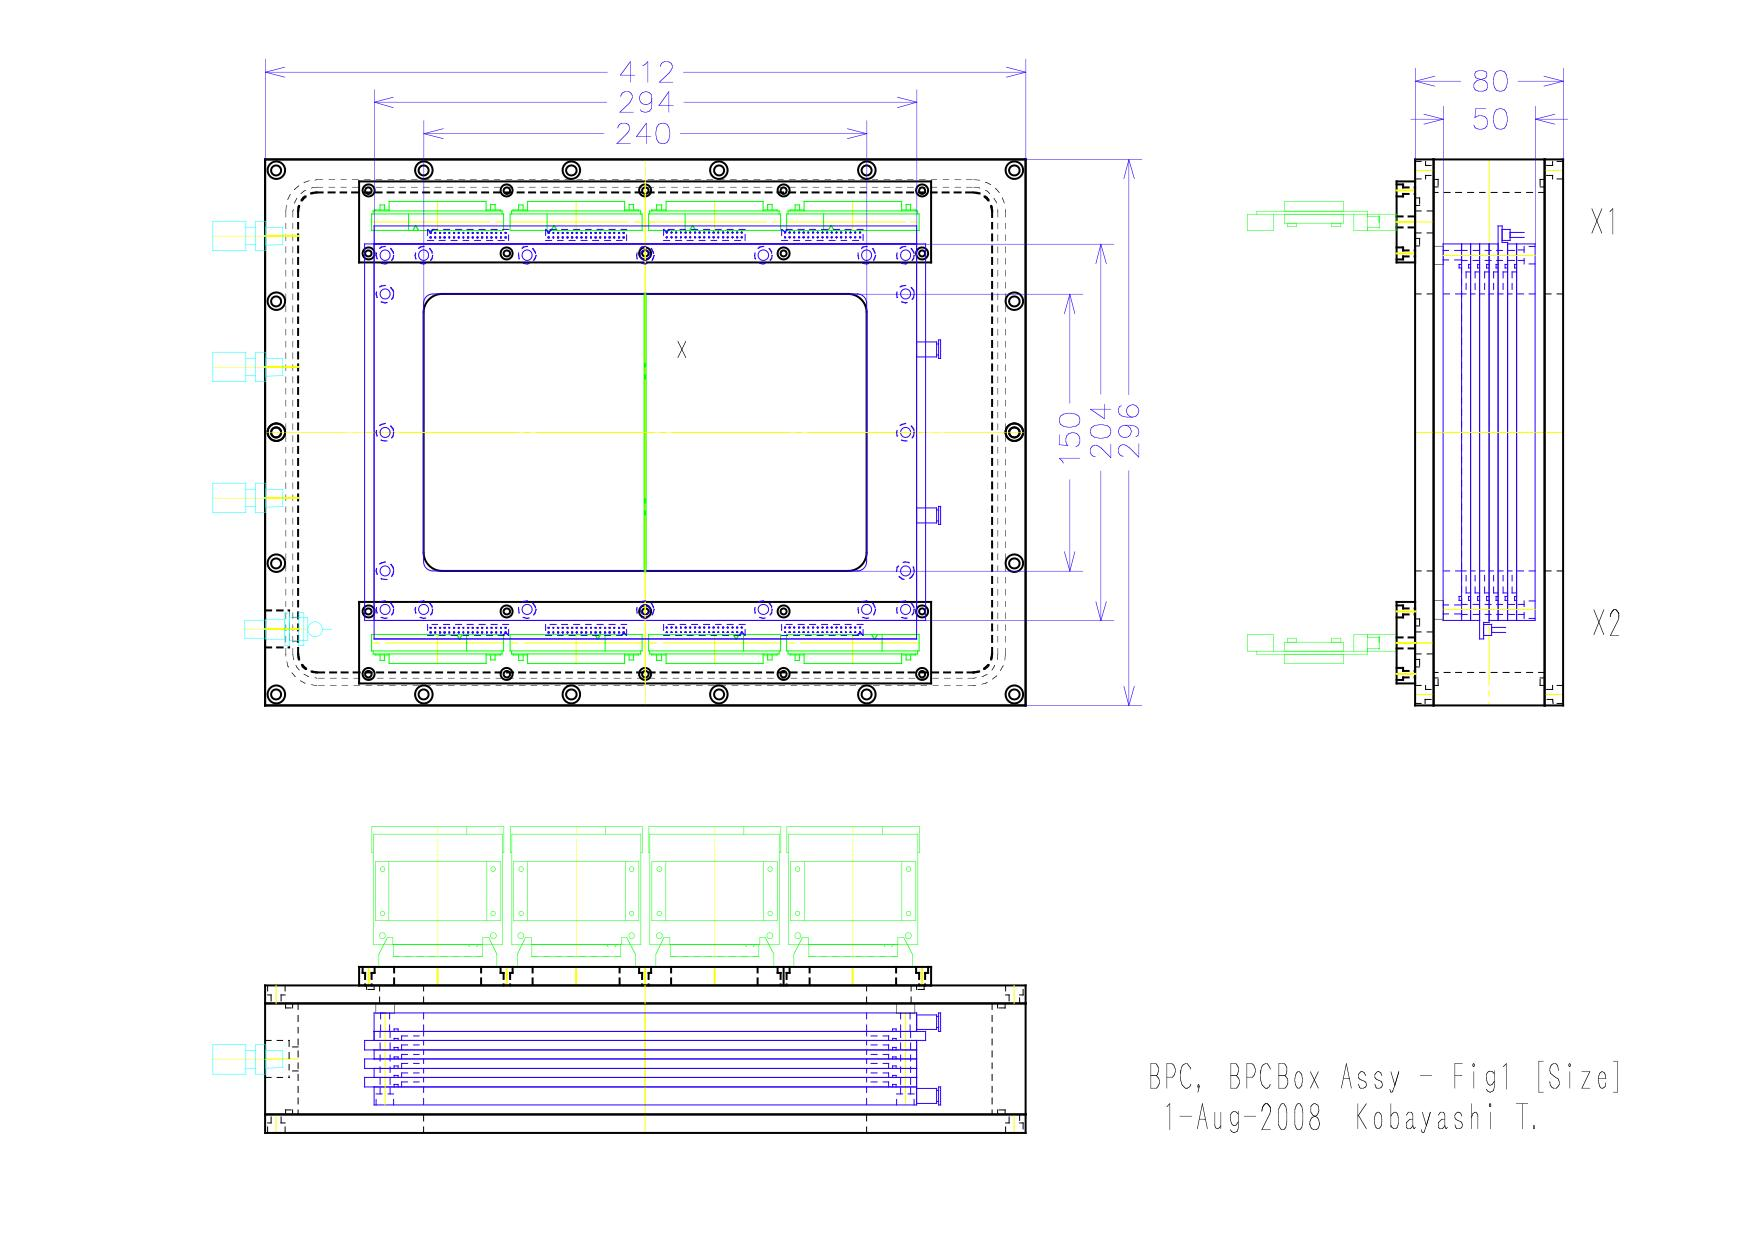
\includegraphics[width=12cm]{chapter3/bpc_a1.jpg}
    \end{subfigure}
    \begin{subfigure}[h]{\textwidth}
        \hspace{2.4cm}
        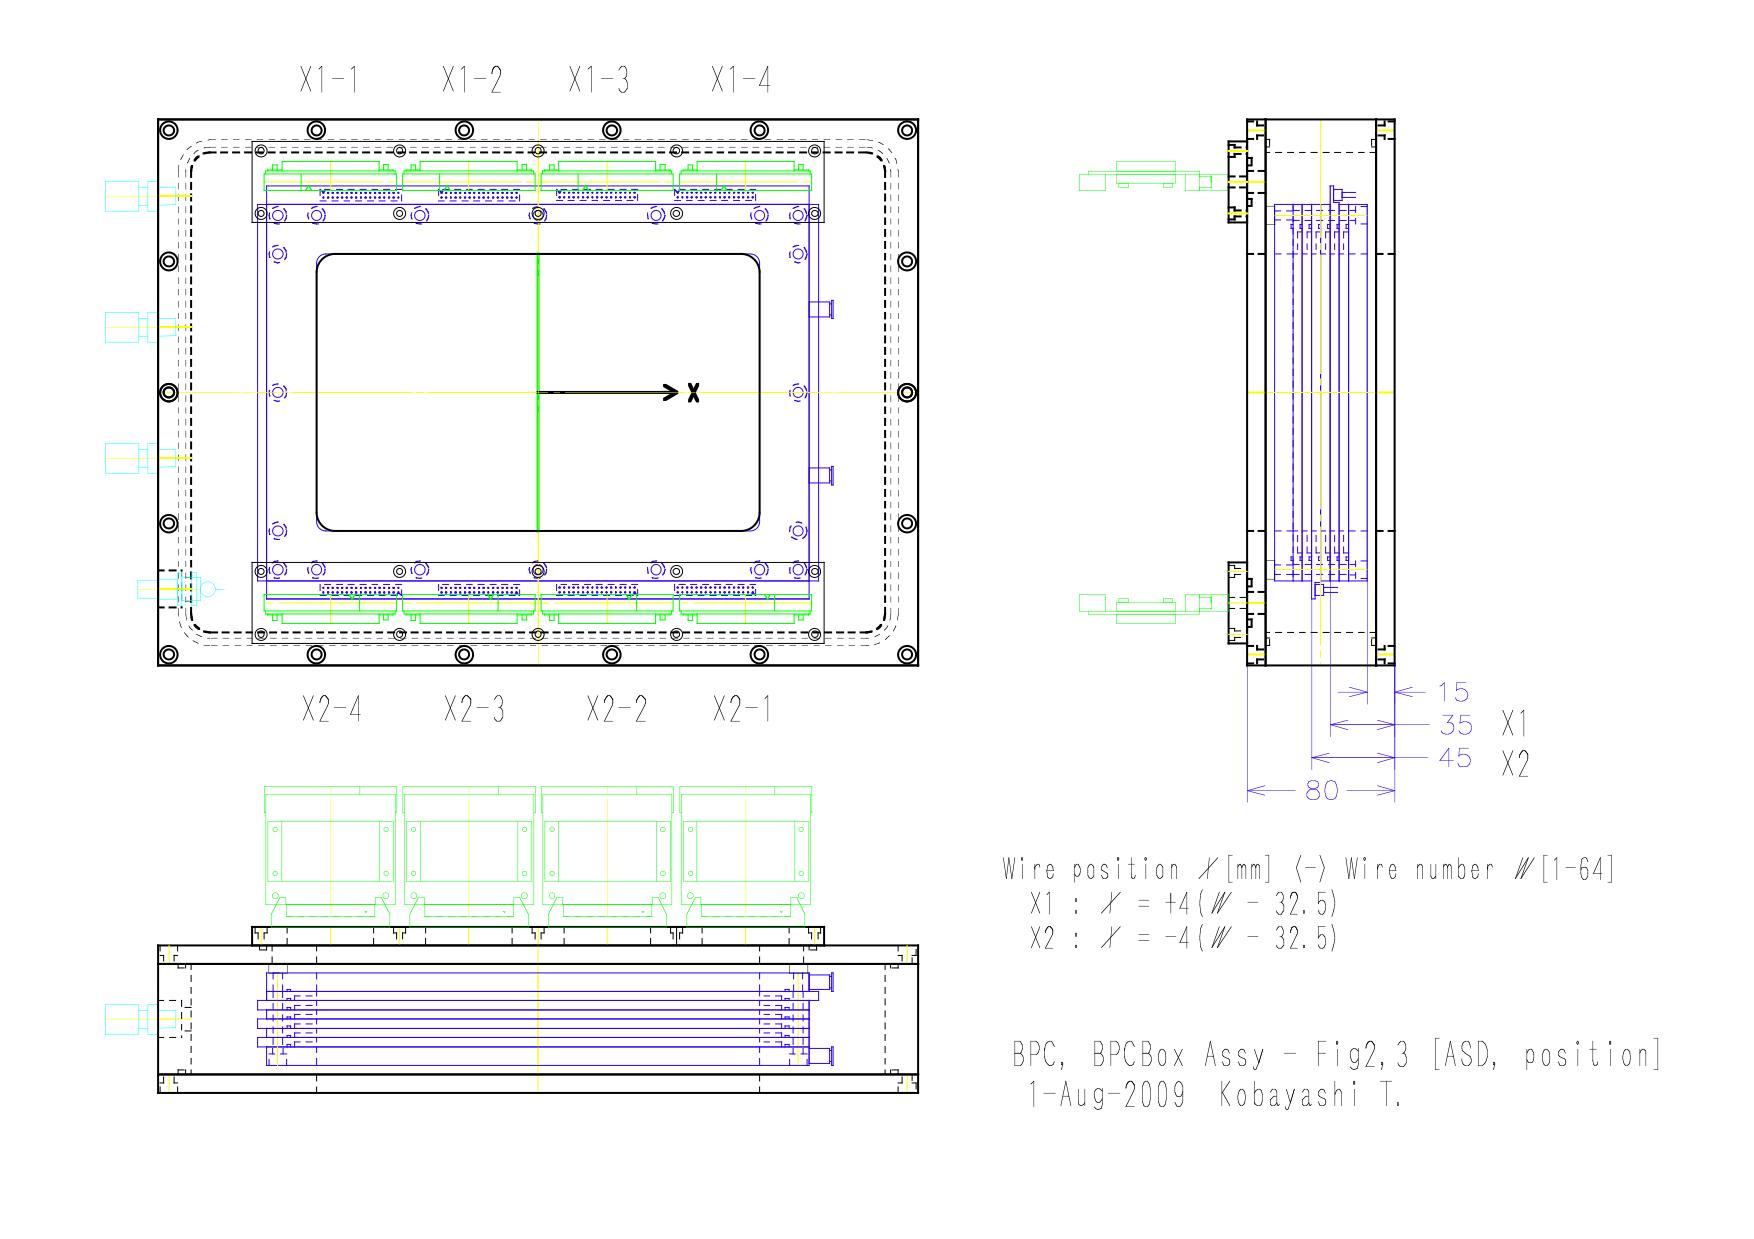
\includegraphics[width=12.5cm]{chapter3/bpc_a23.jpg}
    \end{subfigure}
        \caption{Schematic view of BPC (Beam Proportional Chamber) \cite{SAMURAI}}
        \label{fig:BPC}
\end{figure}

\clearpage

\subsection{ICB (Ion Chamber for Beam)}
The ICB is multi-layer ionization chamber for measuring the energy loss ($\Delta E$) of secondary beam. Using P10 gas at 1 atm, the energy loss of secondary beam can be measured. Figure \ref{fig:ICB} shows the schematic view of ICB and Table \ref{tab:ICB} shows the parameter of ICB.
\begin{table}[h]
    \centering
    \begin{tabular}{l|c}
        \hline
        Effective Area & (H)140mm $\times$ (V)140mm $\times$ (D)420mm\\
        Configuration & 10 anodes and 11 cathodes \\
        Anode-cathode gap & 21mm \\
        Gas & P10 at 1 atm\\
        Distance from target upstream & 4.76 m \\
        \hline
    \end{tabular}
    \caption{Parameter of ICB (Ion Chamber for Beam) \cite{SAMURAI}}
    \label{tab:ICB}
\end{table}

\begin{figure}[t]
    \centering
    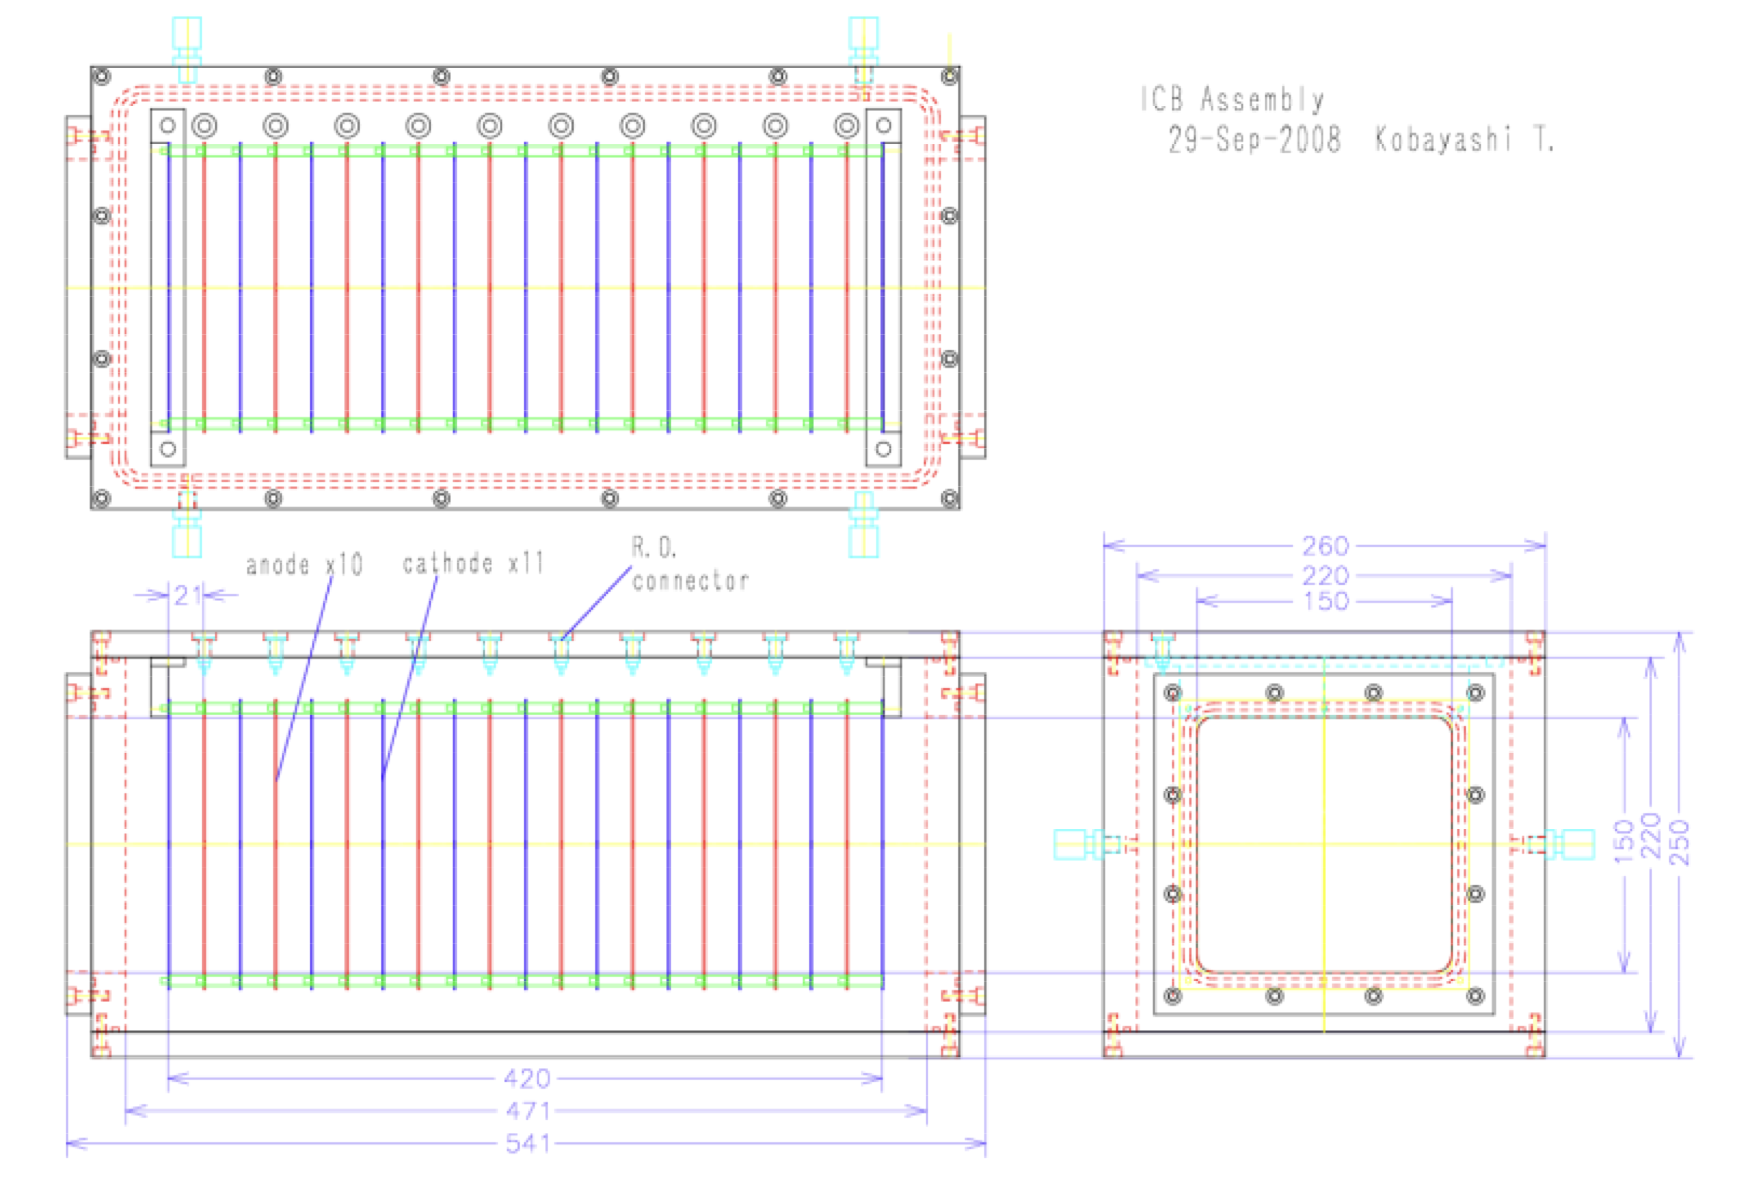
\includegraphics[width=11cm]{chapter3/icb_a}
    \caption{Schematic view of ICB (Ion Chamber for Beam) \cite{SAMURAI}}
    \label{fig:ICB}
\end{figure}

\subsection{BDC1, BDC2 (Beam Drift Chamber)}
Before target, there are two Beam drift chamber for reconstructing the trajectory of secondary beam. Using the trajectory information, the position of secondary beam at target can be calculated. In this experiment, each BDC box is filled with $i$--${C}_{4} {H}_{10}$ gas at 100 torr. Figure \ref{fig:BDC} shows the schematic view of BDC and Table \ref{tab:BDC} shows the parameter of BDC.

\begin{figure}[h]
    \centering
    \begin{subfigure}{\textwidth}
        \centering
        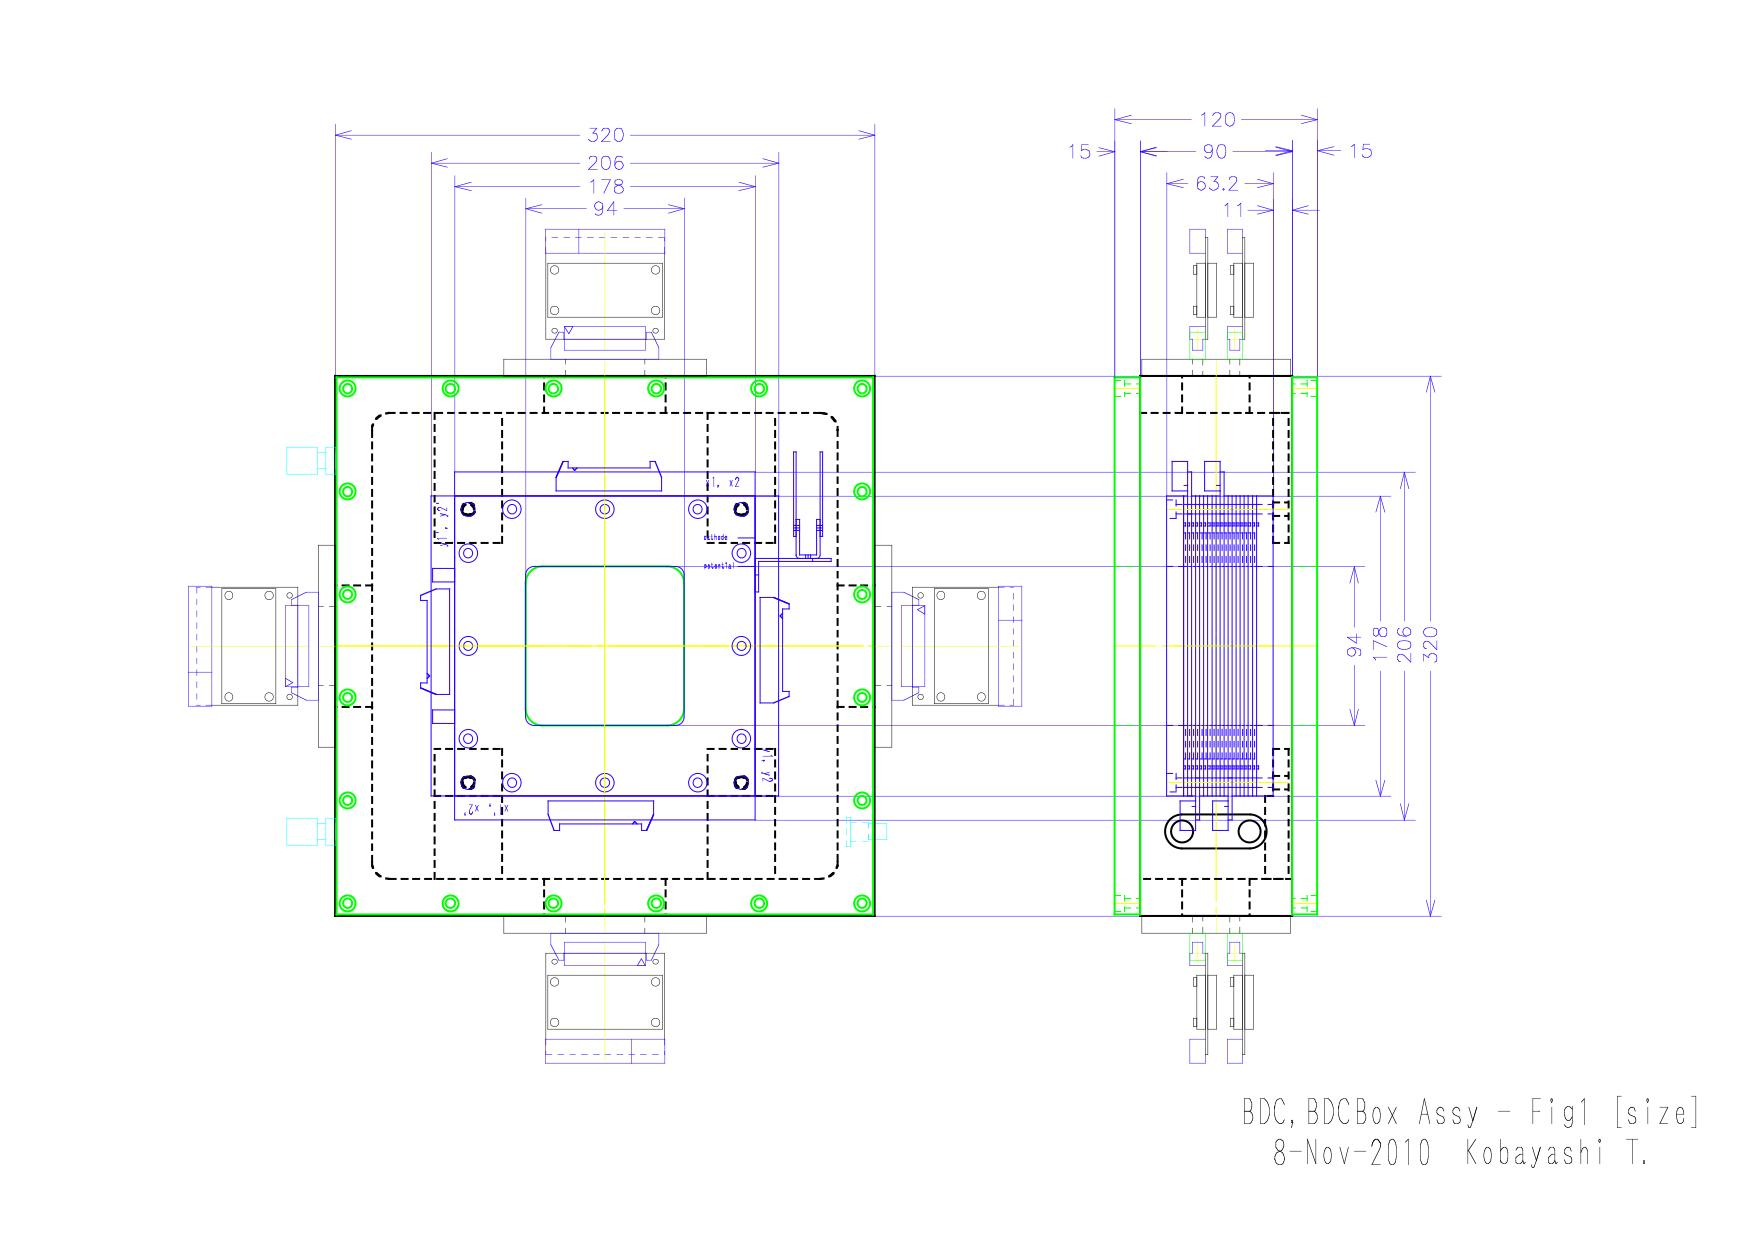
\includegraphics[width=12.5cm]{chapter3/bdc_a1.jpg}    
    \end{subfigure}
    \begin{subfigure}{\textwidth}
        \hspace{1.5cm}
        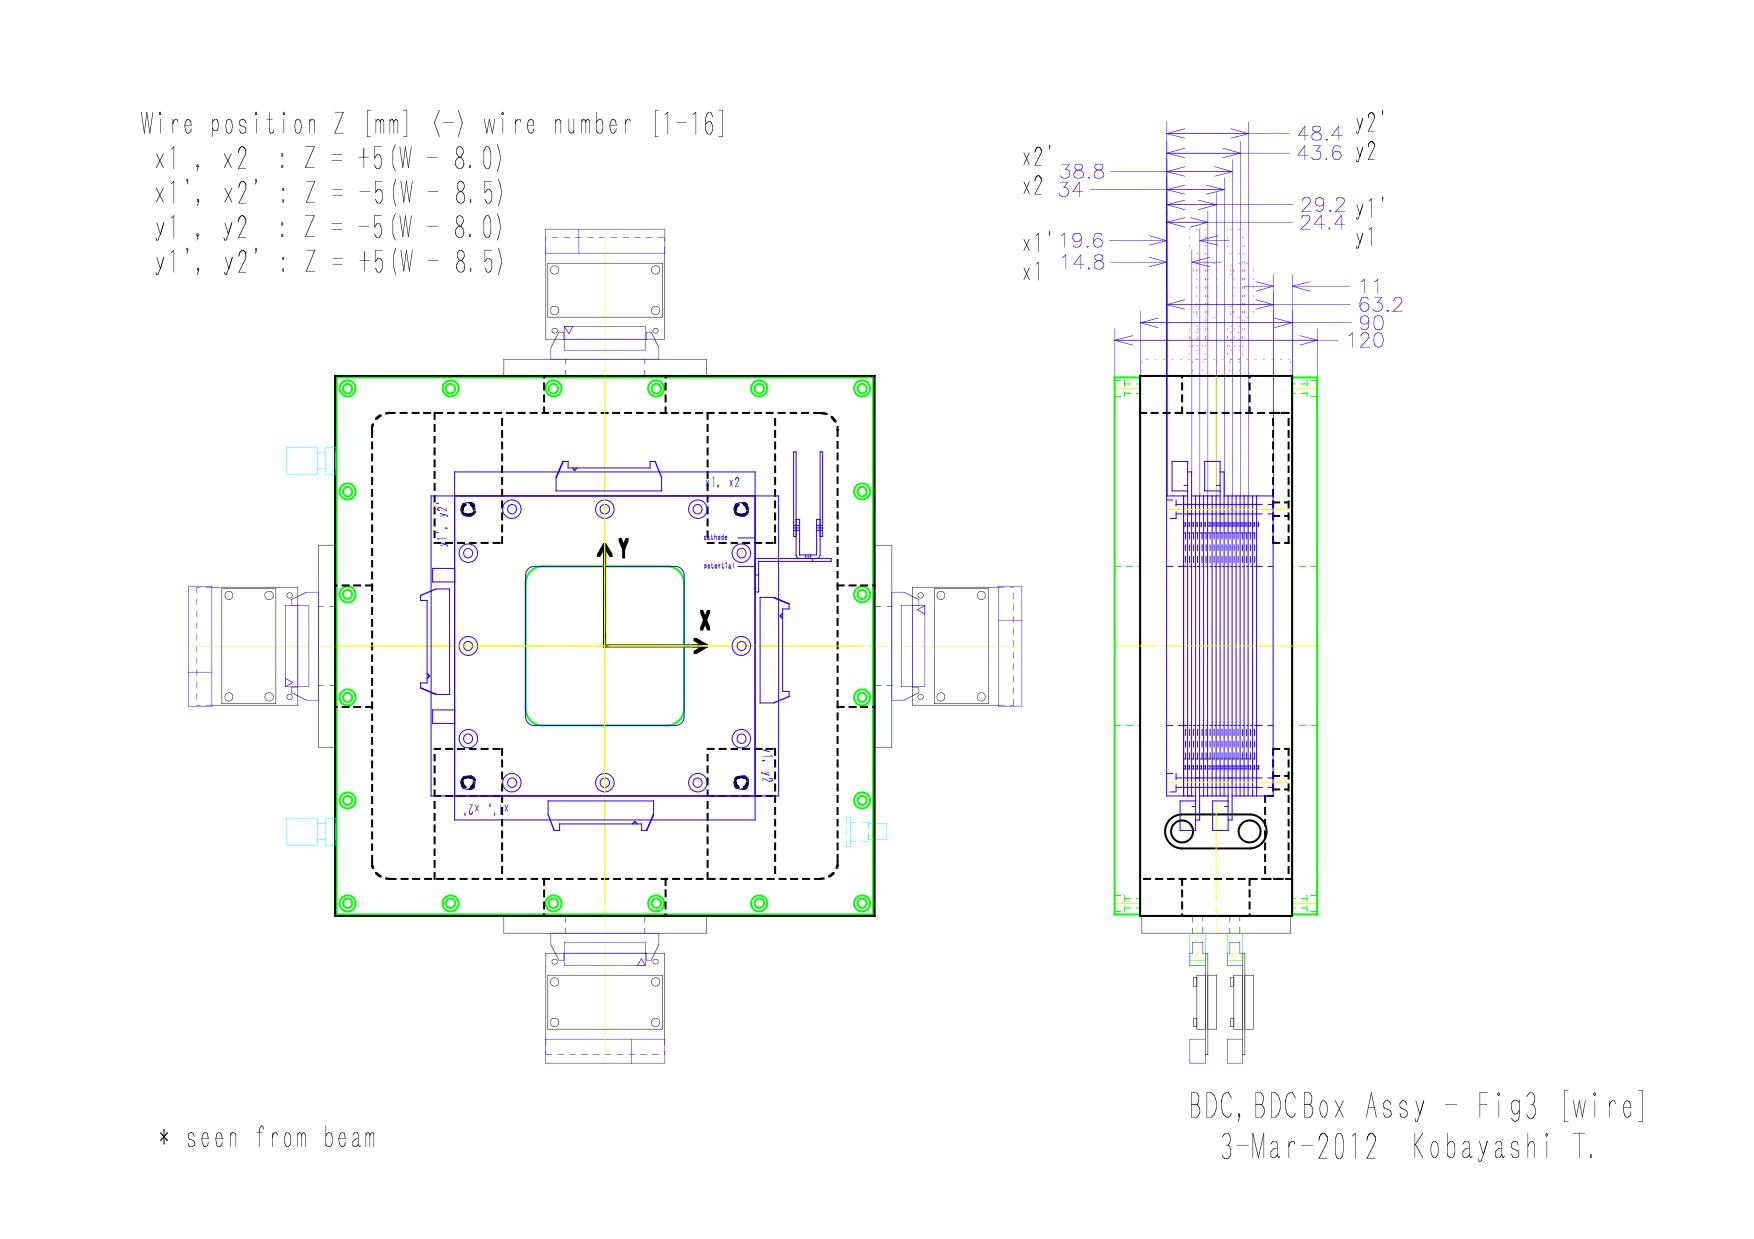
\includegraphics[width=12cm]{chapter3/bdc_a3.jpg}
    \end{subfigure}
    \caption{Schematic view of BDC (Beam Drift Chamber) \cite{SAMURAI}}
    \label{fig:BDC}
\end{figure}

\clearpage
\begin{table}
    \centering
    \begin{tabular}[h]{l|c}
        \hline
        Effective Area & (H)80mm $\times$ (V)80mm\\
        Configuration & $XX'YY'XX'YY'$ (8 planes)\\
        Number of Wire & 16 $\times$ 8 = 128 \\
        Wire Pitch & 5mm \\
        Gas & $i$--${\text{C}}_{4} {\text{H}}_{10}$ at 100 torr\\
        Distance from target upstream & (BDC1) 2.03 m (BDC2) 1.03 m \\
        \hline
    \end{tabular}
    \caption{Parameter of BDC (Beam Drift Chamber) \cite{SAMURAI}}
    \label{tab:BDC}
\end{table}

\subsection{DALI2}
DALI2 (Detector Array for Low Intensity radiation 2) is a NaI(Tl) detector array for $\gamma$-ray spectroscopy\cite{DALI2}. It is consisted of 140 NaI(Tl) crystals surrounding the secondary target. The $\gamma$-ray emitted from the reaction at the target can be detected by DALI2. 

\subsection{SAMURAI Magnet}
SAMURAI Magnet is a superconducting dipole magnet for bending the trajectory of charged fragment. The maximum field of SAMURAI magnet is 3.1 T and the maximum current is 563 A. Table \ref{tab:SAMURAI_Magnet} shows the parameter of SAMURAI magnet.

\begin{table}[h]
    \centering 
    \begin{tabular}{l|c}
    \hline
    Type & Superconducting dipole magnet \\
    Magnet Pole & $\phi$ 2m (0.88 m gap) \\
    Maximum field & 3.1 T \\
    Maximum current & 563 A \\
    %Acceptance & $\theta_H \leq \pm 10{}^{\circ}$, $\theta_V \leq \pm 5{}^{\circ}$\\
    \hline
    \end{tabular}
    \caption{Parameter of SAMURAI Magnet \cite{SAMURAI}}
    \label{tab:SAMURAI_Magnet}
\end{table}

\subsection{FDC1, FDC2 (Forward Drift Chamber)}
After target, there are two forward drift chamber (FDC1, FDC2) for reconstructing the trajectory of charged fragment. Using the trajectory information, the rigidity of charged fragment at target can be calculated. In this experiment, FDC1 is filled with $i$--${\text{C}}_{4} {\text{H}}_{10}$ gas at 50 torr and FDC2 is filled with He + 50\% ${\text{C}}_{2} {\text{H}}_{6}$ gas at 1 atm. Figure \ref{fig:FDC1} and \ref{fig:FDC2} show the schematic view of FDC1 and FDC2. And Table \ref{tab:FDC1} and \ref{tab:FDC2} show the parameter of FDC1 and FDC2.

\begin{figure}[h]
    \centering
    \begin{subfigure}{\textwidth}
        \centering
        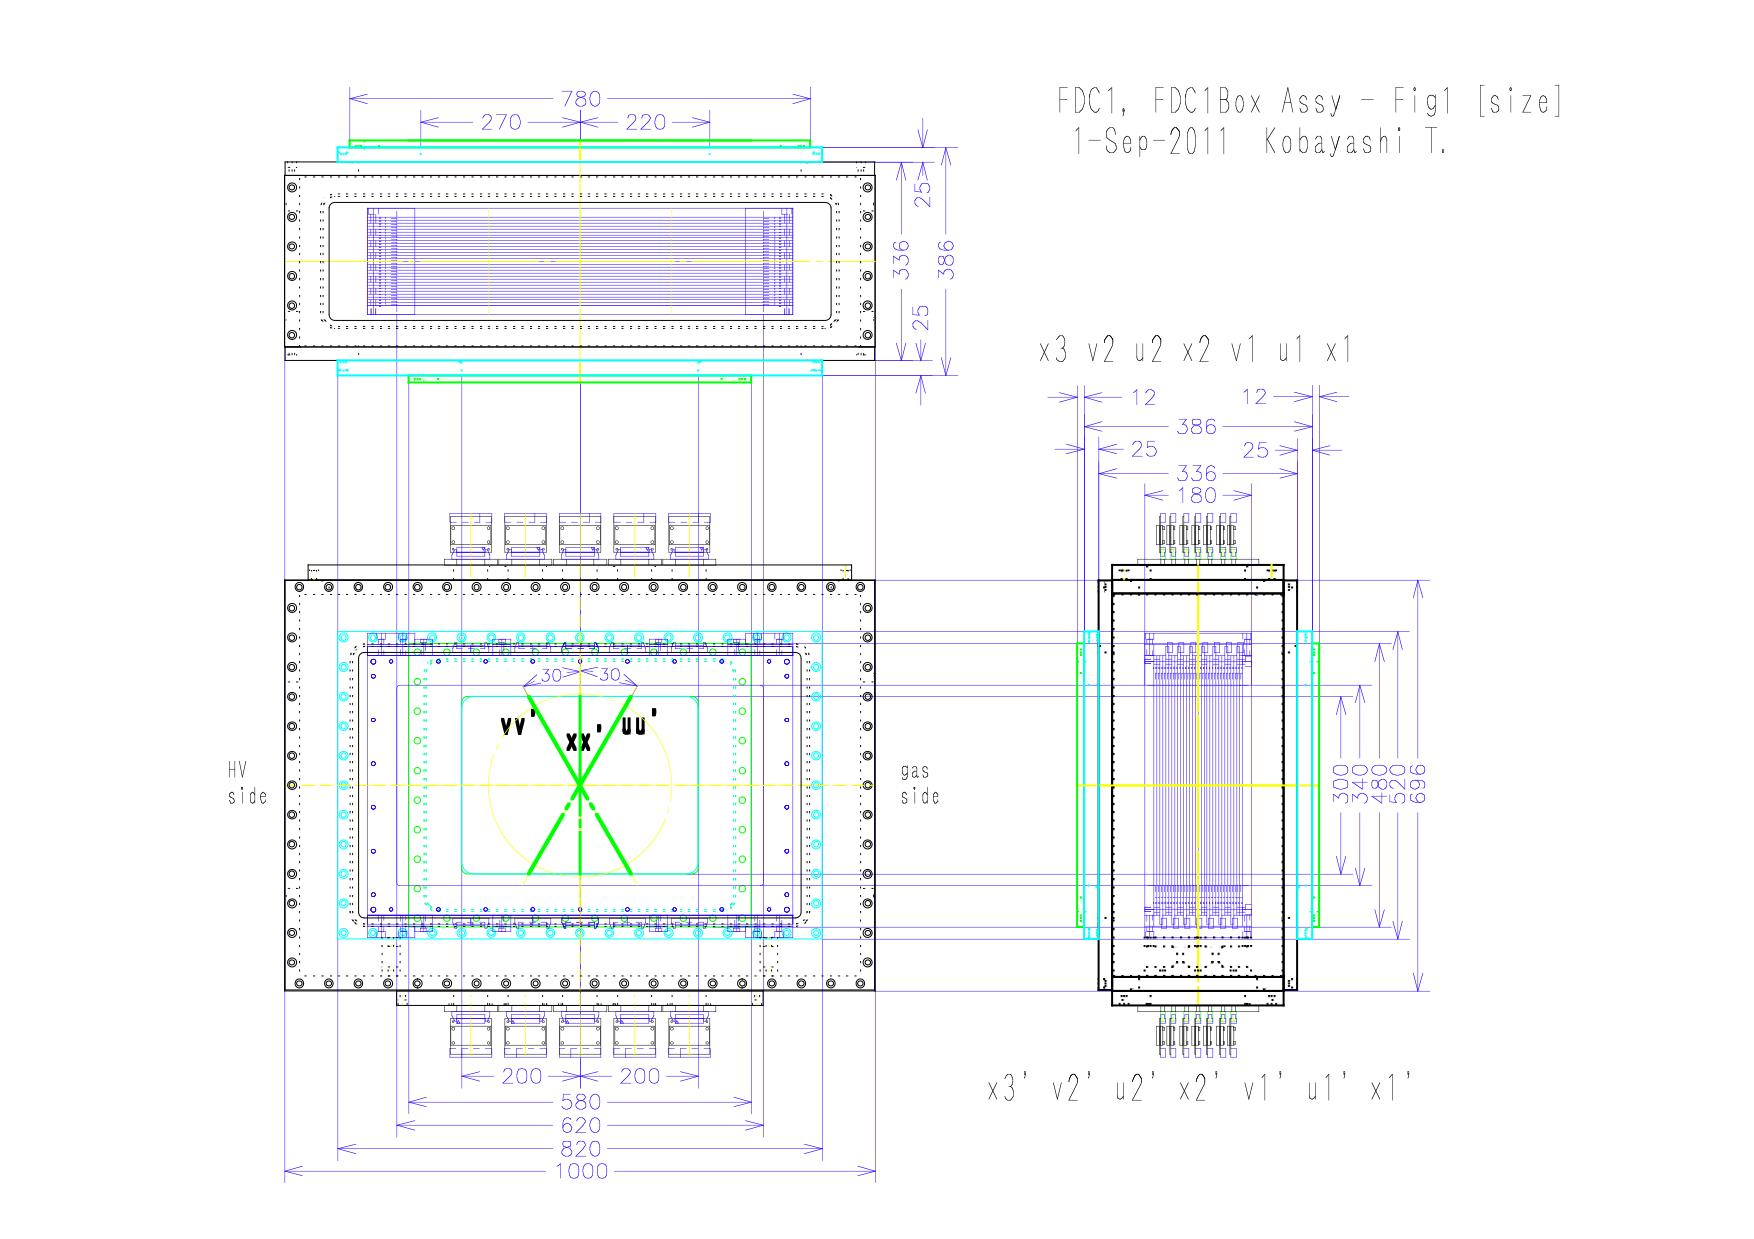
\includegraphics[width=12.5cm]{chapter3/fdc1_a1.jpg}    
    \end{subfigure}
    \begin{subfigure}{\textwidth}
        \hspace{1.5cm}
        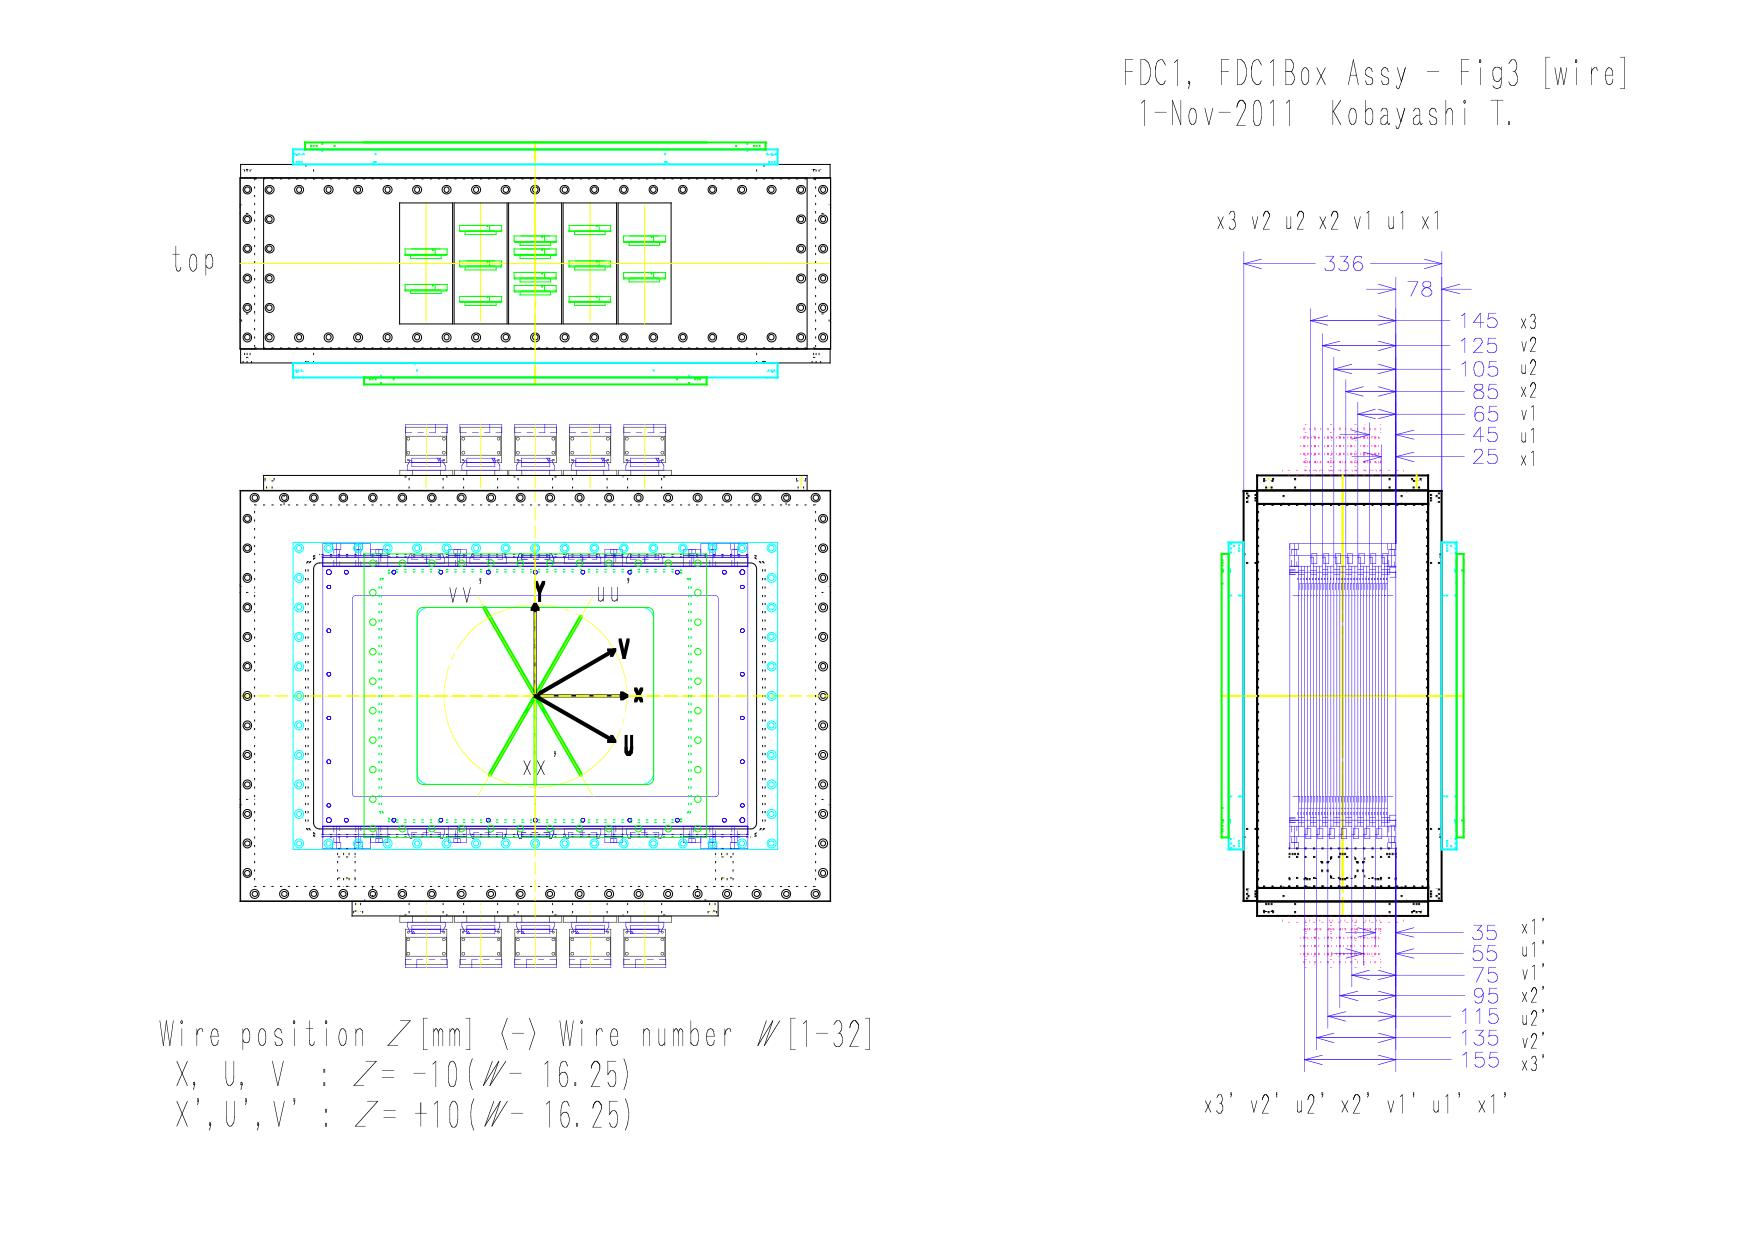
\includegraphics[width=12cm]{chapter3/fdc1_a3.jpg}
    \end{subfigure}
    \caption{Schematic view of FDC1 (Forward Drift Chamber 1) \cite{SAMURAI}}
    \label{fig:FDC1}
\end{figure}
\clearpage

\begin{figure}[h]
    \centering
    \begin{subfigure}{\textwidth}
        \centering
        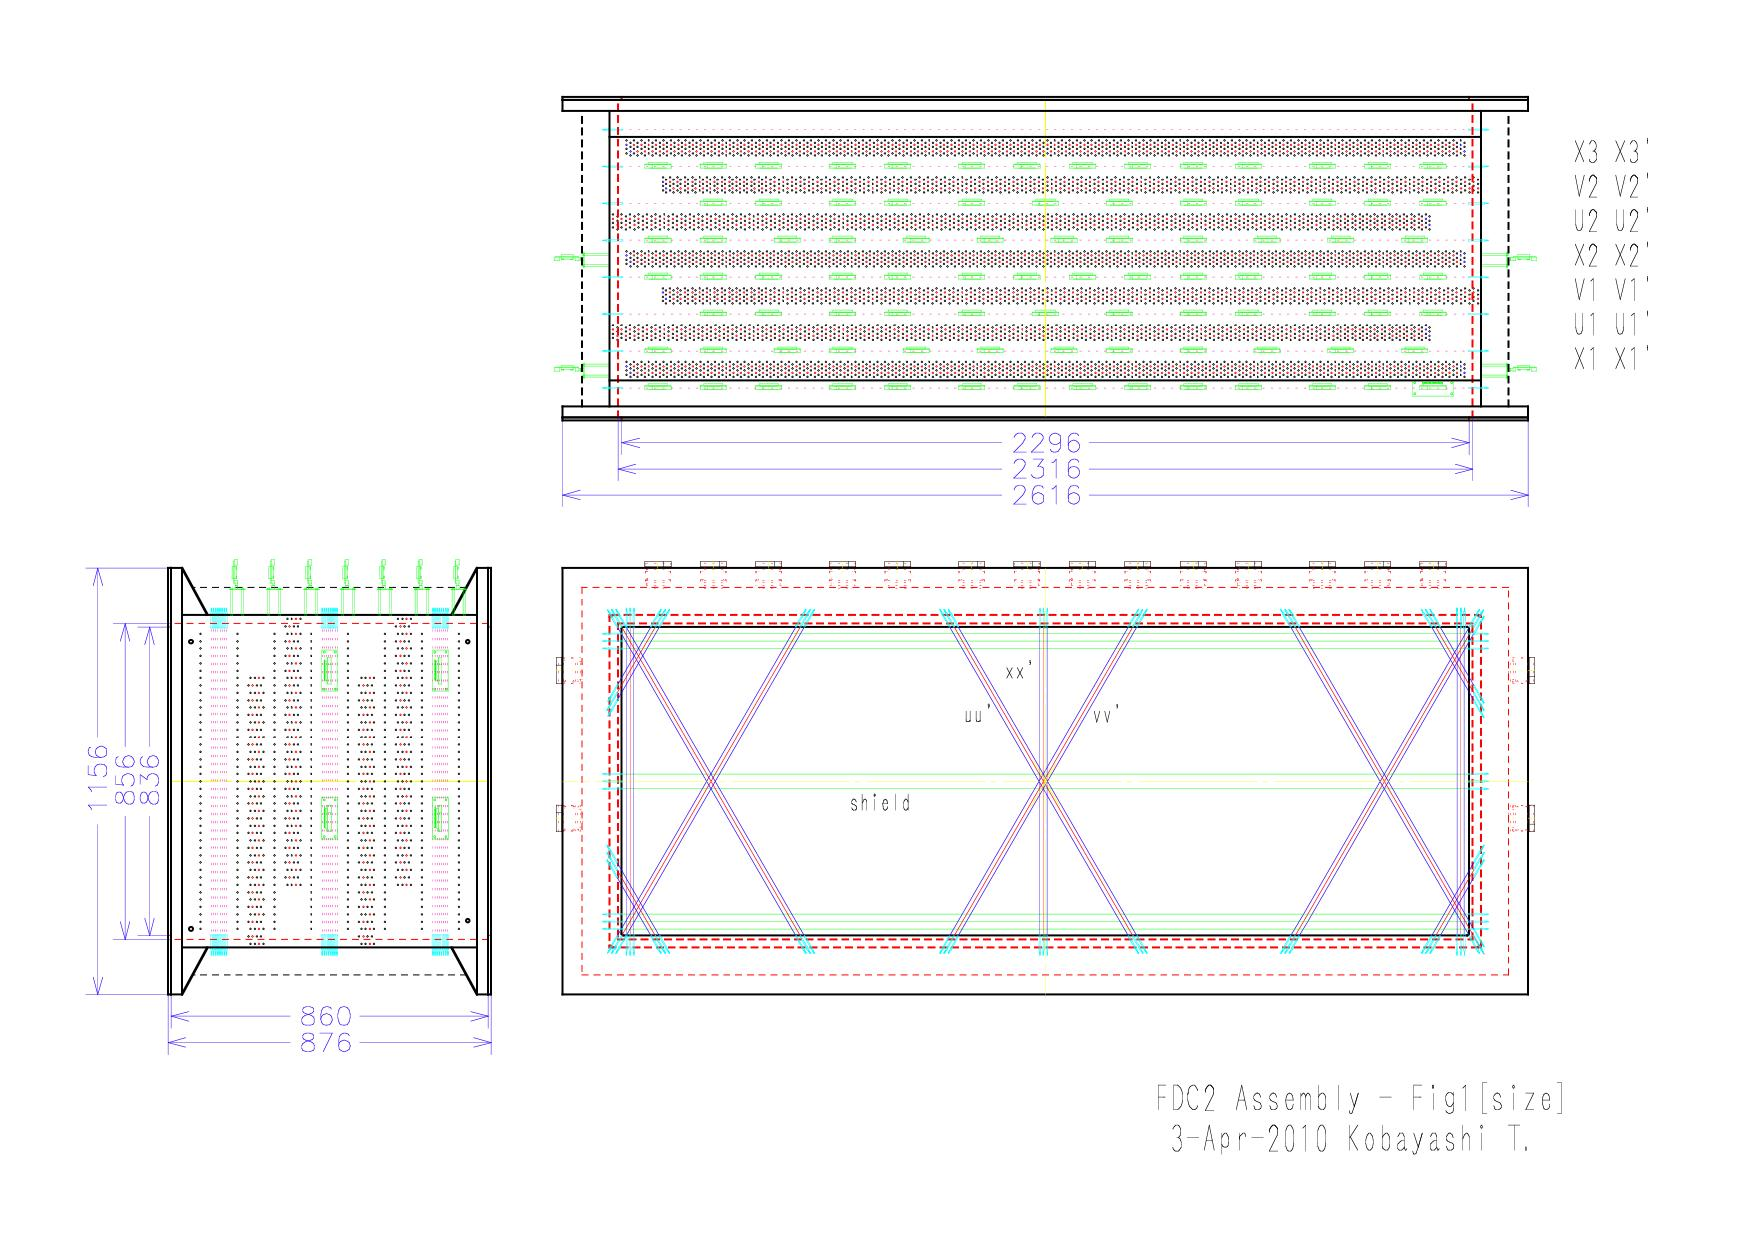
\includegraphics[width=12.5cm]{chapter3/fdc2_a1.jpg}    
    \end{subfigure}
    \begin{subfigure}{\textwidth}
        \hspace{1.5cm}
        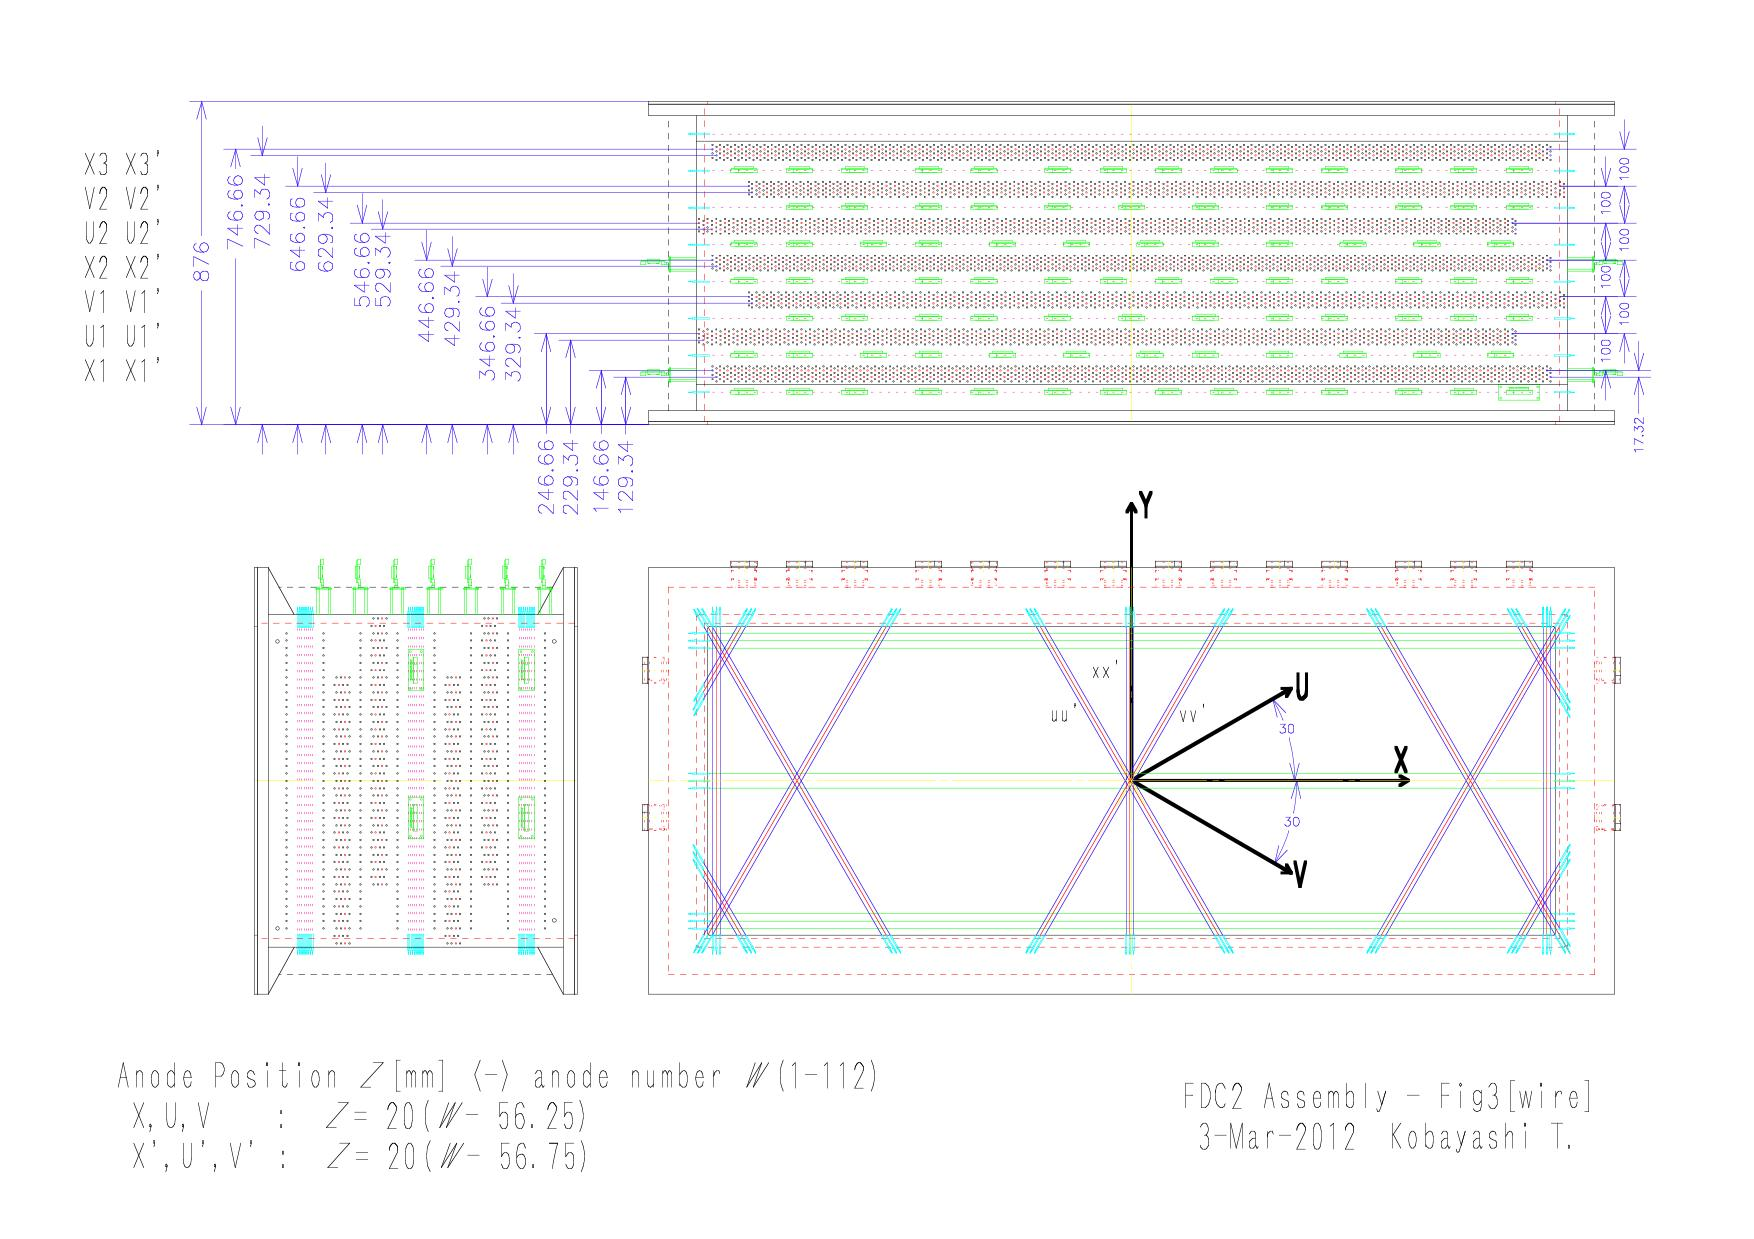
\includegraphics[width=12cm]{chapter3/fdc2_a3.jpg}
    \end{subfigure}
    \caption{Schematic view of FDC2 (Forward Drift Chamber 2) \cite{SAMURAI}}
    \label{fig:FDC2}
\end{figure}
\clearpage

\begin{table}[h]
    \centering
    \begin{tabular}{l|c}
        \hline
        Effective Area & (H)400mm $\times$ (V)300mm $\times$ (D)180mm\\
        Configuration & $XX'UU'VV'XX'UU'VV'XX'$ (14 planes)\\
        Number of Wire & 32 $\times$ 14 = 448 \\
        Wire Pitch & 10mm \\
        Gas & $i$--${C}_{4} {H}_{10}$ at 50 torr\\
        Distance from target upstream & 1151.38 mm  \\
        \hline
    \end{tabular}
    \caption{Parameter of FDC1 (Forward Drift Chamber 1) \cite{SAMURAI}}
    \label{tab:FDC1}
\end{table}

\begin{table}[h]
    \centering
    \begin{tabular}{l|c}
        \hline
        Effective Area & (H)2296mm $\times$ (V)836mm $\times$ (D)860mm\\
        Configuration & $XX'UU'VV'XX'UU'VV'XX'$ (14 planes)\\
        Number of Wire & 112 $\times$ 14 = 1568 \\
        Wire Pitch & 20mm \\
        Gas & He + 50\% ${C}_{2} {H}_{6}$ at 1 atm\\
        \hline
    \end{tabular}
    \caption{Parameter of FDC2 (Forward Drift Chamber 2) \cite{SAMURAI}}
    \label{tab:FDC2}
\end{table}

\subsection{HODF (HODoscope for Fragment)}
The plastic scintillator HODscope is located behind FDC2 for measuring the time of flight (TOF) and energy loss of charged fragment. HODF is consisted of 16 modules of plastic scintillator. Table \ref{tab:HODF} shows the parameter of HODF and Figure \ref{fig:HODF} shows the schematic view of HODF.

\begin{table}[h]
    \centering
    \begin{tabular}{l|c}
        \hline
        Effective Area & (H)1600mm $\times$ (V)1200mm $\times$ (D)10mm\\
        Module & (H)100mm $\times$ (V)1200mm $\times$ (D)10mm\\
        Configuration & 16 module/layer $\times$ 1 layers \\
        \hline
    \end{tabular}
    \caption{Parameter of HODF (HODscope for Fragment) \cite{SAMURAI}}
    \label{tab:HODF}
\end{table}

\clearpage

\begin{figure}[h]
    \centering
    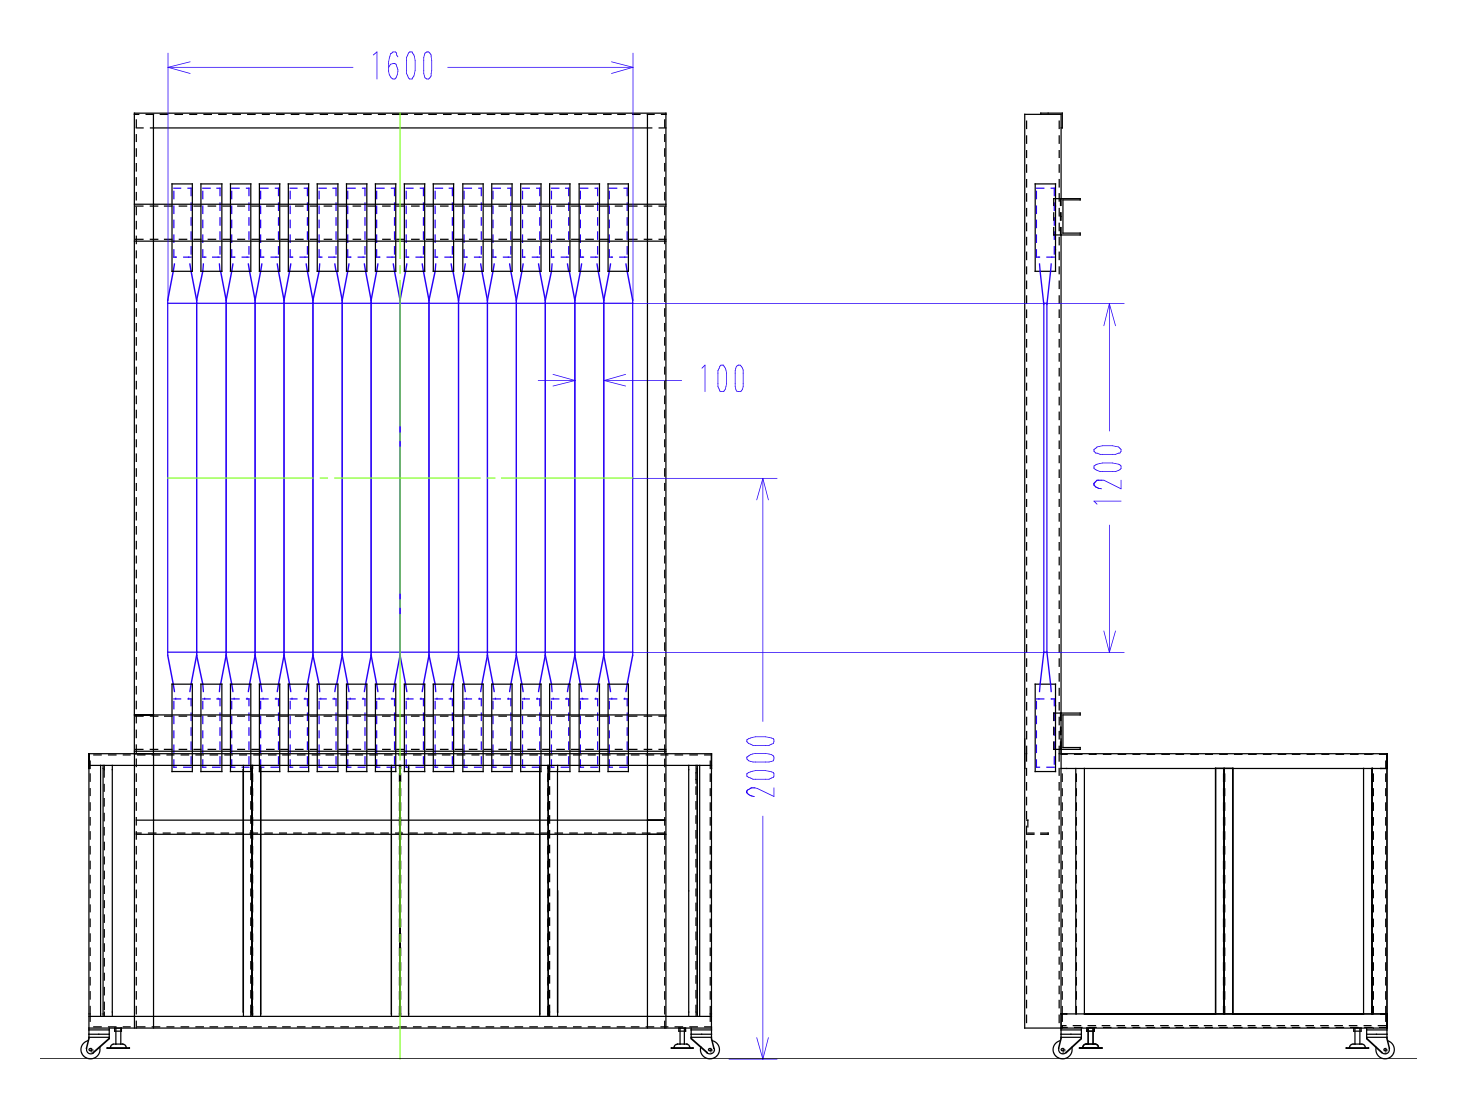
\includegraphics[width=12cm]{chapter3/hodf.png}
    \caption{Schematic view of HODF (HODscope for Fragment) \cite{SAMURAI}}
    \label{fig:HODF}
\end{figure}

\subsection{NEBULA}
NEBULA (NEutron detection system for Break up of Unstable nuclei with Large Acceptance) is a neutron detector array located at the end of the extended beam line. NEBULA is consisted of 120 plastic scintillators for neutron detection and 24 plastic scintillators for veto. By NEBULA, we can reconstructed the neutron momentum vector from the target. Figure \ref{fig:NEBULA} shows the schematic view of NEBULA and Table \ref{tab:NEBULA} shows the parameter of NEBULA.

\begin{table}[h]
    \centering
    \begin{tabular}{l|c}
        \hline
        \multicolumn{2}{c}{Neutron detector}\\
        \hline
        Effective aria & (H)3600mm $\times$ (V)1800mm\\
        Module & (H)120mm $\times$ (D)120mm $\times$ (V)1800mm\\
        Configuration & 30 module/layer $\times$ 4 layers \\
        \hline
        \multicolumn{2}{c}{Veto detector} \\
        \hline
        Effective area & (H)3800mm $\times$ (V)1900mm\\
        Module & (H)320mm $\times$ (D)10mm $\times$ (V)1900mm\\
        Configuration & 12 module/layer $\times$ 2 layers \\
        \hline
    \end{tabular}
    \caption{Parameter of NEBULA \cite{SAMURAI}}
    \label{tab:NEBULA}
\end{table}

\begin{figure}[h]
    \centering
    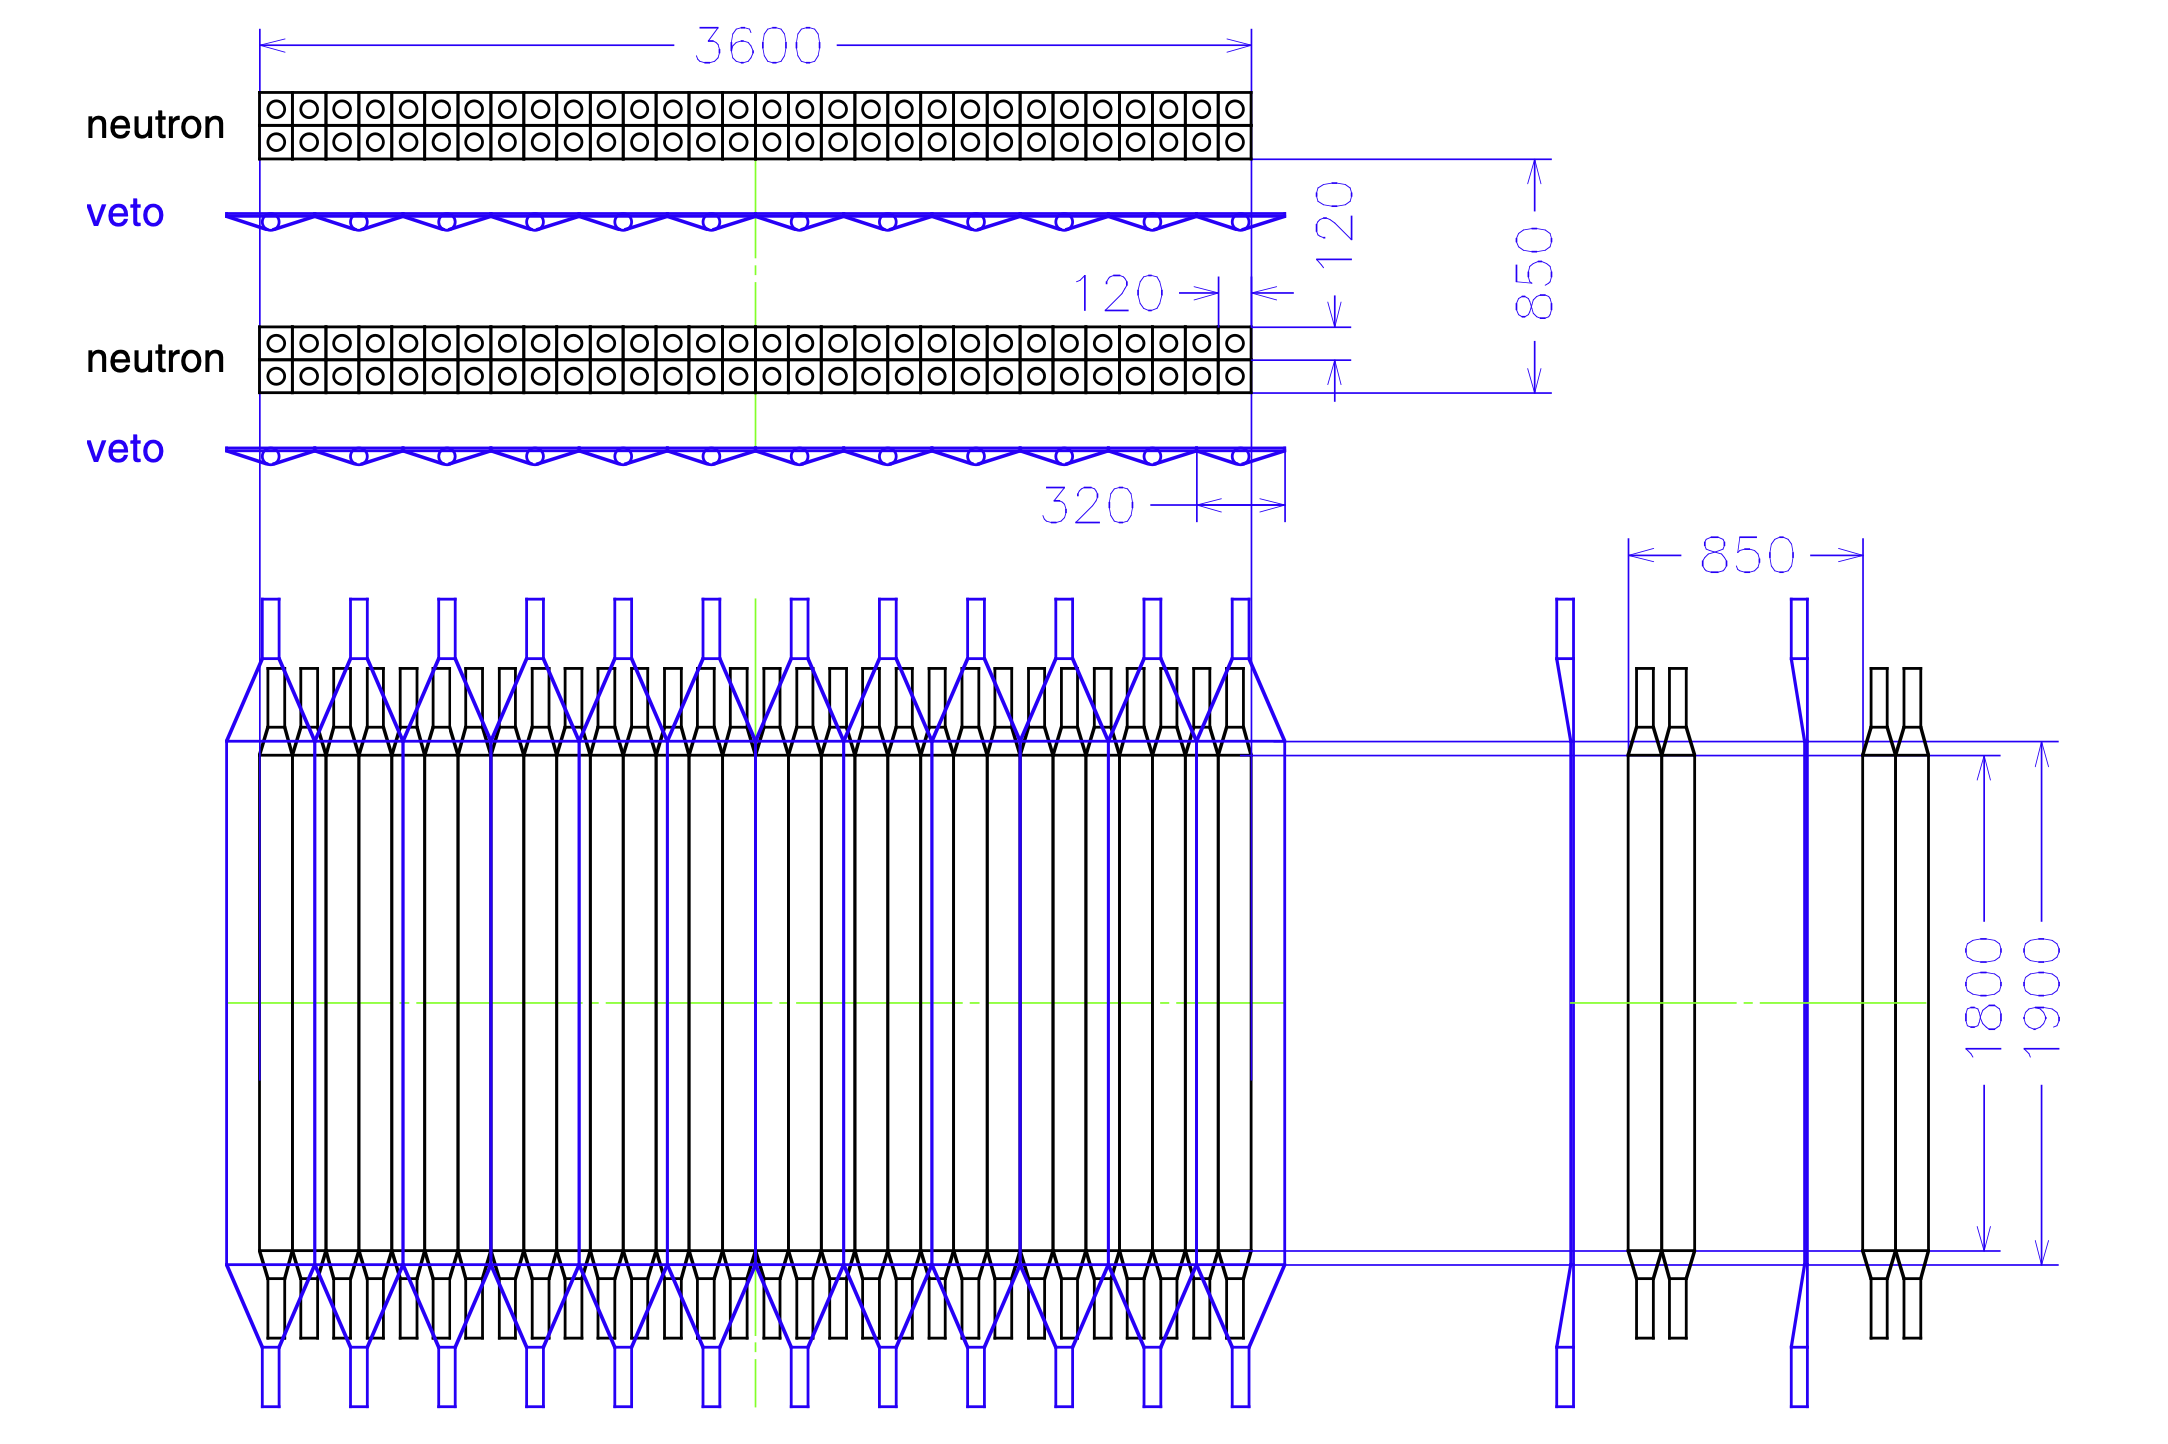
\includegraphics[width=12cm]{chapter3/nebula.png}
    \caption{Schematic view of NEBULA \cite{SAMURAI}}
    \label{fig:NEBULA}
\end{figure}

\subsection{Geometry Information of SAMURAI Setup}
Figure \ref{fig:Geometry} shows the geometry information of SAMURAI setup\cite{Dayonewiki}.

\begin{figure}
    \centering
    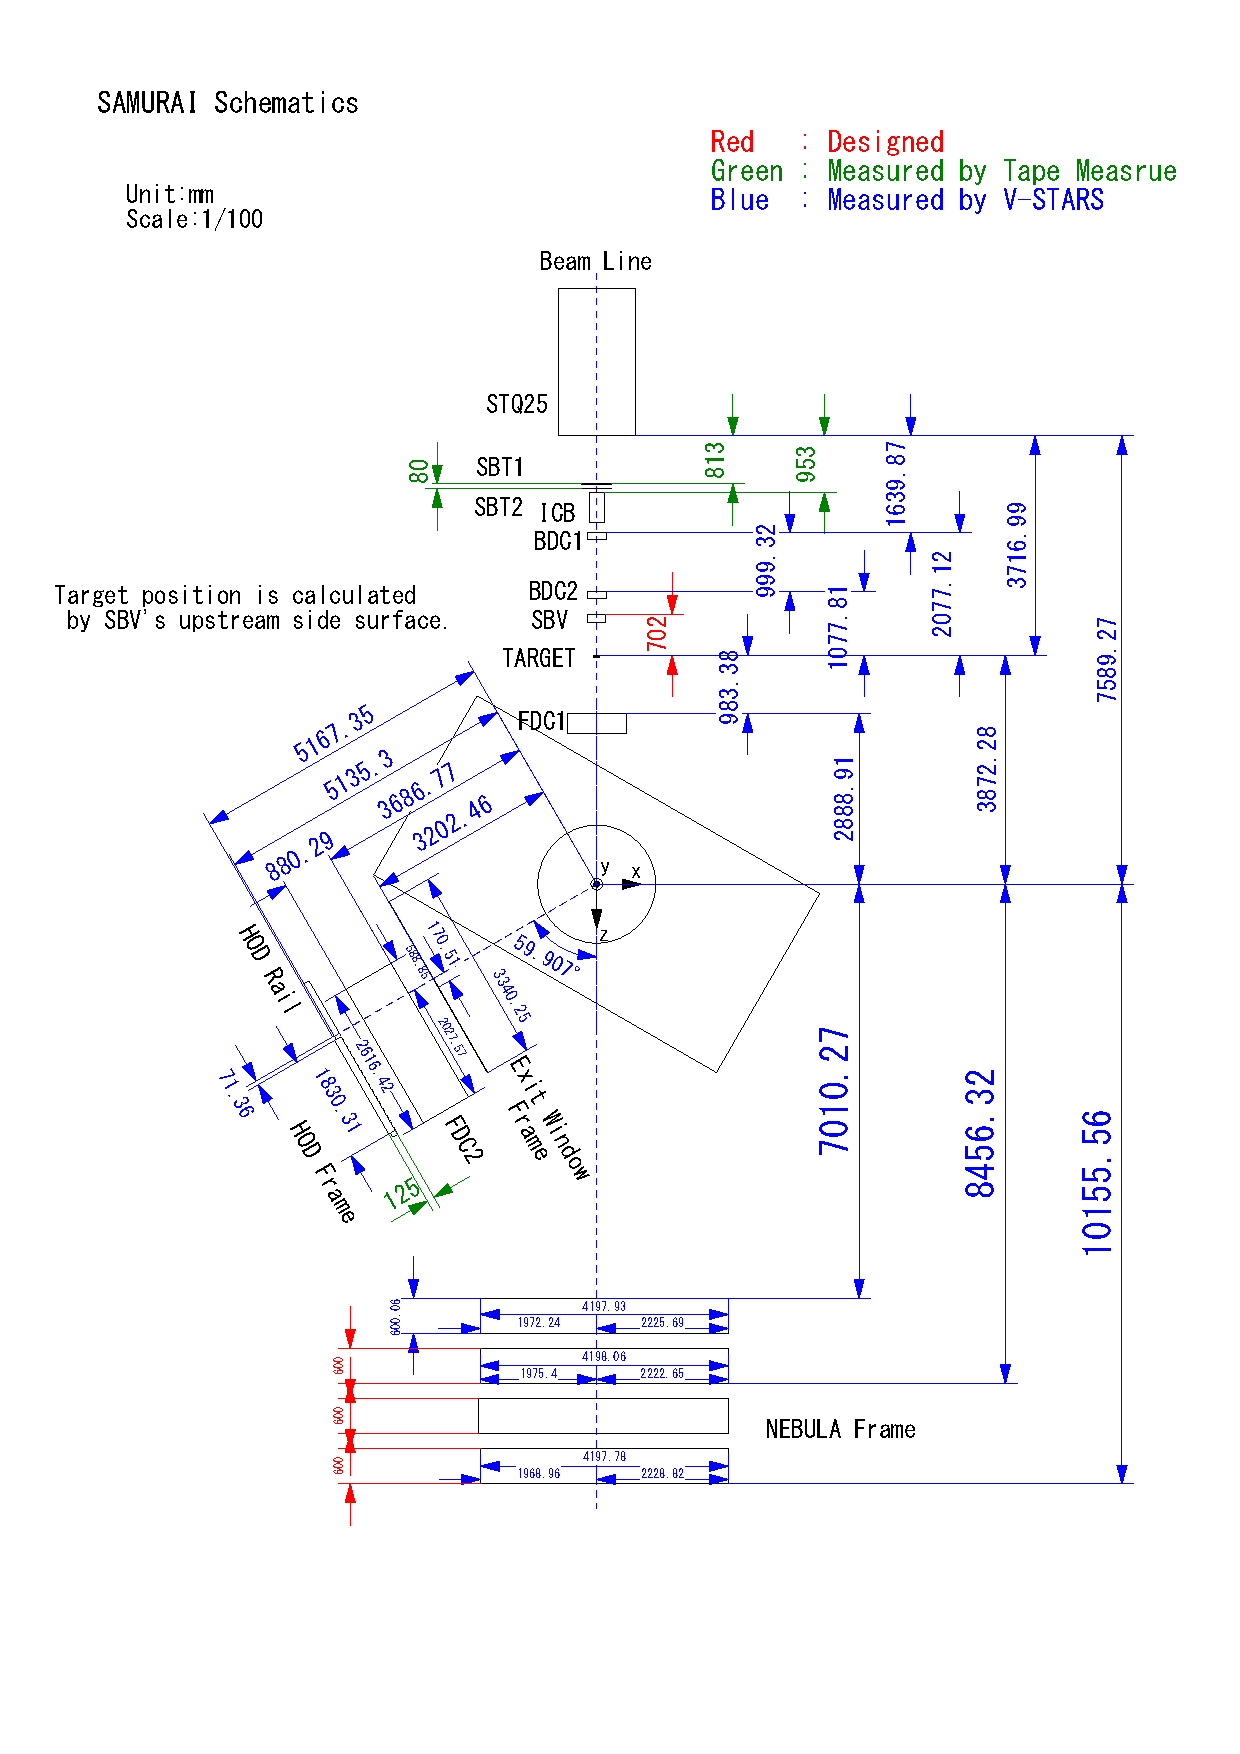
\includegraphics[width=0.9\textwidth]{chapter3/minakata-geometry-drawing_20131121.pdf}
    \caption{Geometry information of SAMURAI setup \cite{Dayonewiki}}
    \label{fig:Geometry}
\end{figure}

\clearpage

\section{Run Summary}
In this thesis, the data from the following runs are used for the data analysis. The run number, target, trigger condition, and note are shown in Table \ref{tab:Run_Summary}.

\begin{table}[h]
    \centering
    \begin{tabular}[h]{c|ccc}
        \hline
        Run number& Target & Trigger & Note\\
        \hline
        394 - 404 &  C (1.789 g/cm${}^{2}$)  & DSB(1/20) $\cup$  (B $\cap$ N) $\cup$ D(1/1) &\\
        405 - 409 &  Empty  & DSB(1/20) $\cup$ (B $\cap$ N) $\cup$ D(1/1) &\\
        410 - 427 &  Pb (3.255 g/cm${}^{2}$)  & DSB(1/20) $\cup$ (B $\cap$ N) $\cup$ D(1/1) &\\
        428, 429, 431 & Pb (3.255 g/cm${}^{2}$)  & DSB(1/1) & F5 slit $\pm$1mm \\
        430 & Pb (3.255 g/cm${}^{2}$)  & DSB(1/1) & F5 slit $\pm$5mm \\
        \hline
    \end{tabular}
    \caption{Run summary for experiment\cite{Dayonewiki}}
    \label{tab:Run_Summary}
\end{table}

\section{Electronics}
\subsection{Data Acquisition System and Trigger condition}
There are three trigger conditions used in this experiment: DSB, B $\cap$ N, B $\cap$ N, B $\cap$ D. DSB (Down Scale Beam) trigger means the trigger rate is reduced with the down scale factor. In this research, the physics data set is collected with the down scale factor 1/20. B $\cap$ N (Beam $\cap$ NEBULA) trigger means the coincident between the beam trigger and the NEBULA trigger. B $\cap$ D (Beam $\cap$ DALI) trigger means the coincident between the beam trigger and the DALI trigger. The logic diagrams for beam, NEBULA and DALI trigger condition are shown in Figure \ref{fig:Beam_Trigger}, \ref{fig:NEB_Trigger}, and \ref{fig:DALI_Trigger}. 

\begin{figure}[h]
    \centering
    \hspace{0.5cm}
    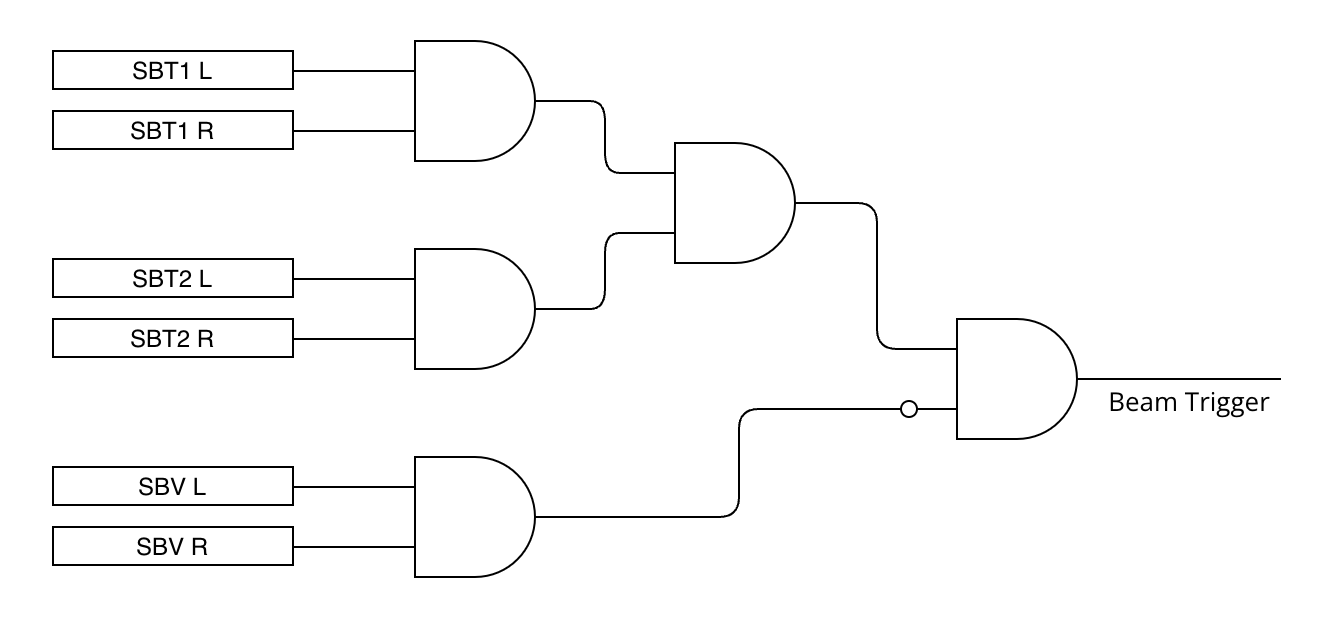
\includegraphics[width=12cm]{chapter3/Beam_Trigger.png}
    \caption{Logic diagram for beam trigger}
    \label{fig:Beam_Trigger}
\end{figure}

\begin{figure}[h]
    \centering
    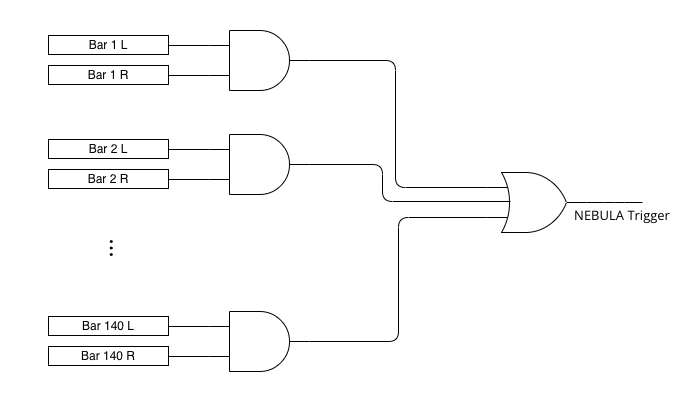
\includegraphics[width=12cm]{chapter3/NEB_Trigger.png}
    \caption{Logic diagram for NEBULA trigger}    
    \label{fig:NEB_Trigger}
\end{figure}

\clearpage

\begin{figure}[h]
    \centering
    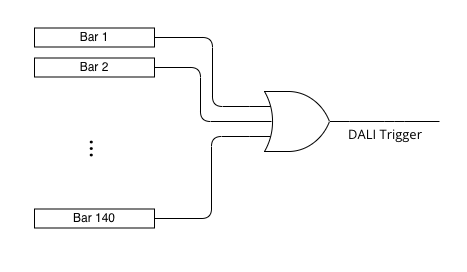
\includegraphics[width=8cm]{chapter3/DALI_Trigger.png}
    \caption{Logic diagram for DALI trigger}
    \label{fig:DALI_Trigger}
\end{figure}


\subsection{Live Time}
The DAQ readout rate is limited by the dead time of the DAQ sub-system and the dead time depends on the trigger condition and the target. Figure \ref{fig:LiveTime} shows the live time of each reaction trigger for the live time correction of cross section.

\begin{table}[h]
    \centering
    \begin{tabular}{c|c|cc}
        \hline
        Run number & target & DSB & B $\cap$ N, B $\cap$ D \\
        \hline
        394 - 404 & C & 0.843 & 0.815 \\
        405 - 409 & Empty & 0.890 & 0.854 \\
        410 - 427 & Pb & 0.861 & 0.831 \\
        \hline
    \end{tabular}
    \caption{Live time of each reaction trigger}
    \label{fig:LiveTime}
\end{table}
